\documentclass[12pt]{article}


\usepackage{showkeys}
\usepackage{hyperref}
\usepackage{amsmath, amssymb, amsthm, bm}
\usepackage[sort&compress,numbers]{natbib}
\usepackage{doi}
\usepackage[margin=1in]{geometry}
\usepackage[all]{xy}
\usepackage{mathrsfs} 
\usepackage{xcolor}
%\textheight23cm \topmargin-20mm  
%\textwidth175mm  
%\oddsidemargin=0mm
%\evensidemargin=0mm
%

\usepackage{amsmath, amsthm, mathtools}

\newtheorem{lemma}{Lemma}
\newtheorem{theorem}{Theorem}
\newtheorem{coro}{Corollary}
\newtheorem{prop}{Proposition}


\theoremstyle{definition}
\newtheorem{defi}{Definition}


\theoremstyle{remark}
\newtheorem{remark}{Remark}
\newtheorem{exm}{Example}

\def\Indep{+^L}

\def\indep{+^L}
\def\cover{\ll}
\def\aff{\operatorname{Aff}}
\def\lin{\operatorname{Lin}}
\def\Span{\operatorname{Span}}
\def\type{\mathrm {setting}}
\def\ii{\bm{\emptyset}}
\def\tt{\bm{0}}
\def\Ce{\mathcal C}
\def\Ae{\mathcal A}
\def\Me{\mathcal M}
\def\Le{\mathcal L}
\def\Te{\mathcal T}
\def\Fe{\mathcal F}
\def\Pe{\mathcal P}
\def \Tr{\mathrm{Tr}\,}
\def\Se {\mathcal S}
\def\supp{\mathrm{supp}}
\def\permut{\mathscr{S}}

\def\<{\langle\,}
\def\>{\,\rangle}
%\def \BS{\mathrm{BS}}
\def\vtl{\vartriangleleft}
\def\vtr{\vartriangleright}
\def \Afh{\mathrm{AfH}}
\def \Af{\mathrm{Af}}
\def \FV{\mathrm{FinVect}}
\def\bV{\mathbf V}
\def\bW{\mathbf W}
\def\bE{ E}
\def\bI{I}

\def\Cl{\mathrm{Clas}}
\def\Quant{\mathrm{Quant}}
\def\bX{ X}
\def\bQ{\mathbf Q}
\def\bY{ Y}
\def\bZ{Z}

\makeatletter

\newcommand*\@bigplus[1]{\vcenter{\hbox{#1$\m@th +$}}}
\newcommand*\bigplus{%
    \DOTSB % omit this line if you are not using the amsmath package
    \mathop{%
        \mathchoice
            {\@bigplus \huge}%
            {\@bigplus \LARGE}%
            {\@bigplus {}}%
            {\@bigplus \footnotesize}%
    }%
    \slimits@ % omit this line if you are not using the amsmath package
}

\makeatother




\title{On the structure of  higher order quantum maps}
\author{Anna Jen\v cov\'a}

\begin{document}

\maketitle

\section{Affine subspaces and higher order maps}

\subsection{The category $\FV$} \label{sec:fv}


The category $\FV$ is a basic  example of a compact closed category, whose structure
underlies all the results in this paper. For basics on category theory and symmetric
monoidal categories, see [MacLane]. For compact closed categories and the use of categories in quantum theory, see
[book]. [Kelly compact closed] 



Let  $\FV$ be the category of finite dimensional real vector spaces with linear maps. 
We will denote the usual tensor product by $\otimes$, then  $(\FV,\otimes, I=\mathbb R)$
is a symmetric monoidal category, with the associators, unitors and symmetries given by
the obvious isomorphisms 
\begin{align*}
\alpha_{U,V,W}&:(U\otimes V)\otimes W\simeq U\otimes (V\otimes W), \\
\lambda_V&: I\otimes
V\simeq
V, \qquad \rho_V: V\otimes I\simeq V,\\
\sigma_{U,V}&: U\otimes V\simeq V\otimes U.
\end{align*}



Let  $(-)^*: V\mapsto V^*$ be the usual vector space dual, with duality denoted by
$\<\cdot,\cdot\>: V^*\times V\to \mathbb R$. We will use the canonical identification
$V^{**}=V$ and $(V_1\otimes V_2)^*=V_1^*\otimes V_2^*$. With this duality, $\FV$ is
compact closed. This means that for each object $V$, there are morphisms $\eta_V: I\to V^*\otimes
V$ (the ''cup'') and $\epsilon_V: V\otimes V^*\to I$ (the ''cap'') such that the following snake
identities hold:
\begin{equation}\label{eq:snake}
(\epsilon_V\otimes V)\circ (V\otimes \eta_V)=V,\qquad (V^*\otimes \epsilon_V)\circ
(\eta_V\otimes V^*)=V^*,
\end{equation}
here we denote the identity map on the object $V$ by $V$. 



Let us identify these morphisms.
First, $\eta_V$ is a linear map $\mathbb R\to V^*\otimes V$, which can be
identified with the element $\eta_V(1)\in V^*\otimes V$ and   $\epsilon_V\in (V\otimes
V^*)^*=V^*\otimes V$ is again an element of the same space.  Choose a basis
$\{e_i\}$ of $V$, let $\{e_i^*\}$ be the dual basis of $V^*$, that is,
$\<e_i^*,e_j\>=\delta_{i,j}$. Let us define
\[
\eta_V(1)=\epsilon_V:=\sum_i e_i^*\otimes e_i.
\]
It is easy to see that this definition does not depend on the choice of the basis, indeed,
$\epsilon_V$ is the linear functional on $V\otimes V^*$ defined by
\[
\<\epsilon_V, x\otimes x^*\>=\<x^*,x\>,\qquad x\in V, \ x^*\in V^*.
\]
It is also easily checked that the snake identities \eqref{eq:snake} hold.

For two objects $V$ and $W$ in $\FV$, we will denote the set of all morphisms (i.e. linear
maps) $V\to
W$ by $\FV(V,W)$. Then $\FV(V,W)$ is itself a real linear space and  we have the well-known identification 
$\FV(V,W)\simeq V^*\otimes W$. This can be given as follows: for each $f\in \FV(V,W)$, we have 
$C_f:=(V^*\otimes f)(\epsilon_V)=\sum_i e_i^*\otimes f(e_i)\in V^*\otimes W$. Conversely,
since $\{e_i^*\}$ is a basis of $V^*$, 
any element $w\in V^*\otimes W$ can be uniquely written as $w=\sum_i e_i^*\otimes w_i$ for
$w_i\in W$, and since $\{e_i\}$ is a basis of $V$, the assignment $f(e_i):=w_i$ determines a
unique map $f:V\to W$. The relations between $f\in \FV(V,W)$ and $C_f\in V^*\otimes W$ can
be also written as
\[
\<C_f,x\otimes y^*\>=\<\epsilon_V,x\otimes f^*(y^*)\>=\<f^*(y^*),x\>=\<y^*,f(x)\>,\qquad x\in
V,\ y^*\in W^*,
\]
here $f^*:W^*\to V^*$ is the adjoint of $f$.
Note that by compactness, the {\em internal hom} in $\FV$ satisfies $V\multimap W\simeq V^*\otimes W$,
so that  in the case of $\FV$, the object $V\multimap W$ can be identified with the space of linear
maps $\FV(V,W)$. 

The following two examples  are most important for us.

\begin{exm}\label{exm:classical} Let $V=\mathbb R^N$. In this case, we fix the canonical basis $\{|i\>,\
i=1,\dots,N\}$. We will identify $(\mathbb R^N)^*=\mathbb R^N$, with duality
$\<x,y\>=\sum_i x_iy_i$, in particular, we identify $I=I^*$. We then have
$\epsilon_V=\sum_i |i\>\otimes |i\>$ and if $f:\mathbb R^N\to \mathbb R^M$ is given by the
matrix $A$ in the two canonical bases, then  $C_f=\sum_i |i\>\otimes A|i\>$ is the
vectorization of $A$.

\end{exm}


\begin{exm}\label{exm:quantum} Let $V=M_n^h$ be the space of $n\times n$ complex hermitian matrices. We again
identify $(M_n^h)^*=M_n^h$, with duality $\<A,B\>=\Tr A^TB$, where $A^T$ is the usual
transpose of the matrix $A$. Let us choose the basis in $M_n^h$, given as
\[
\left\{|j\>\<k|+|k\>\<j|,\ j\le k,\ i\biggl(|j\>\<k|-|k\>\<j|\biggr),\ j<k\right\}.
\]
Then one can check that
\[
\left\{\frac12\biggl(|j\>\<k|+|k\>\<j|\biggl),\ j\le k,\
\frac{i}{2}\biggl(|k\>\<j|-|j\>\<k|\biggr),\ j<k\right\}
\]
is the dual basis and we have
\[
\epsilon_V=\sum_{j,k} |j\>\<k|\otimes |j\>\<k|.
\]
For any $f:M_n^h\to M_m^h$, 
\[
C_f=\sum_{j,k} |j\>\<k|\otimes f(|j\>\<k|)
\]
is the Choi matrix of $f$.

\end{exm}





\subsection{The category $\Af$}

We now introduce the category $\Af$, whose objects  are of the form $X=(V_X,A_X)$, where
$V_X$ is an object in $\FV$  and $A_X\subseteq V_X$ is a proper affine subspace, see Appendix
\ref{sec:app_affine} for definitions and basic properties. Morphisms $X\xrightarrow{f} Y$ in $\Af$ are linear maps $f:V_X\to V_Y$  such that
$f(A_X)\subseteq A_Y$. For two objects $X$ and $Y$ and a  linear map $f:V_X\to V_Y$, we write $X\xrightarrow{f} Y$ with
the meaning that $f$ is a morphism in $\Af$. In particular, if $V_X=V_Y=V$, then  $X\xrightarrow{id_V} Y$ means
that  $A_X\subseteq A_Y$. The set of all morphisms $X\xrightarrow{f} Y$ in $\Af$ will be
denoted by $\Af(X,Y)$.


For any object $X$, we put
\begin{align*}
L_X:=\lin(A_X), \quad  S_X:=\Span(A_X), \quad D_X=\dim(V_X),\quad d_X=\dim(L_X).
\end{align*}
We have
\begin{equation}\label{eq:ALS}
A_X=a+L_X=S_X\cap \{\tilde a\}^{\sim},
\end{equation}
for any choice of elements $a\in A_X$ and $\tilde a\in A^*_X$.


We will next introduce a monoidal structure $\otimes$ as follows. For two objects $X$ and
$Y$, we put  $V_{X\otimes Y}=V_X\otimes V_Y$ and construct the affine subspace
$A_{X\otimes Y}$ as the affine span of 
\[
A_X\otimes A_Y=\{a\otimes b,\ a\in A_X,\ b\in A_Y\}.
\]
Fix any $\tilde a_X\in A^*_X$ and $\tilde a_Y\in A^*_Y$. 
Since $A_X\otimes A_Y\subseteq \{\tilde a_X\otimes \tilde a_Y\}^*$, the affine span of
$A_X\otimes A_Y$ is a proper affine subspace and we have by Lemma \ref{lemma:dual}
\[
A_{X\otimes Y}:=\aff(A_X\otimes A_Y)=\{A_X\otimes A_Y\}^{**}.
\]
\begin{lemma}\label{lemma:tensor_spaces}
For any $a_X\in A_X$, $a_Y\in A_Y$, we  have
\begin{align}
L_{X\otimes Y}&=\lin(A_X\otimes A_Y)=\Span(\{x\otimes y-a_X\otimes a_Y,\ x\in A_X,\ y\in
A_Y\})\label{eq:lxy1}\\
&= (a_X\otimes L_Y)+ (L_X\otimes a_Y)+ (L_X\otimes L_Y)\label{eq:lxy}
%\\ &= S_X\otimes L_Y+L_X\otimes a_Y=a_X\otimes L_Y+L_X\otimes S_Y
\end{align}
(here $+$ denotes the direct sum of subspaces). We also have
\[
S_{X\otimes Y}=S_X\otimes S_Y.
\]
\end{lemma}

\begin{proof} The equality \eqref{eq:lxy1} follows from Lemma \ref{lemma:dual}. For any $x\in A_X$, $y\in A_Y$
 we have
\[
x\otimes y-a_X\otimes a_Y=a_X\otimes (y-a_Y)+(x-a_X)\otimes a_Y+(x-a_X)\otimes (y-a_Y),
\]
so that $L_{X\otimes Y}=\lin(A_X\otimes A_Y)$ is contained in the subspace on the RHS of \eqref{eq:lxy}.
Let $d$ be the dimension of this subspace, then clearly
\[
d_{X\otimes Y}\le d\le d_X+d_Y+d_Xd_Y.
\]
On the other hand, any element of $S_X$ has the form $tx$ for some $t\in \mathbb R$ and
$x\in A_X$, so that it is easily seen that $S_X\otimes S_Y=S_{X\otimes Y}$. 
Hence 
\begin{align*}
d_{X\otimes Y}&=\dim(L_{X\otimes Y})=\dim(S_{X\otimes
Y})-1=\dim(S_X)\dim(S_Y)-1=(d_X+1)(d_Y+1)-1\\
&=d_X+d_Y+d_Xd_Y.
\end{align*}
This completes the proof.

\end{proof}




\begin{lemma}\label{lemma:monoidal} Let $I=(\mathbb R,\{1\})$. Then 
$(\Af,\otimes, I)$ is a symmetric monoidal category.
\end{lemma}

\begin{proof} Note that this structure is inherited from the symmetric monoidal structure
in $\FV$. To show that $\otimes$ is a functor, we have to check that for $X_1\xrightarrow{f} Y_1$ and $X_2\xrightarrow{g} Y_2$ in
$\Af$, we have $X_1\otimes Y_1\xrightarrow{f\otimes g} X_2\otimes Y_2$ which amounts to
showing that 
\[
(f\otimes g)(A_{X_1\otimes Y_1})\subseteq A_{X_2\otimes Y_2}.
\]
Let $x\in A_{X_1}$, $y\in A_{Y_1}$, then $f(x)\otimes g(y)\in A_{X_2}\otimes
A_{Y_2}\subseteq A_{X_2\otimes Y_2}$. Since  $A_{X_1\otimes Y_1}$ is the affine subspace
generated by $A_{X_1}\otimes A_{Y_1}$, the above inclusion follows by linearity of $f\otimes
g$. 

It only remains to prove that the associators, unitors and symmetries from
$\FV$ are morphisms in $\Af$. We will prove this for the associators $\alpha_{X,Y,Z}:V_X\otimes (V_Y\otimes V_Z)\to
(V_X\otimes V_Y)\otimes V_Z$, the other proofs are similar. We need to check that
$\alpha_{X,Y,Z}(A_{X\otimes(Y\otimes Z)})\subseteq A_{(X\otimes Y)\otimes Z}$. It is easily
checked that $A_{X\otimes(Y\otimes Z)}$ is the affine span of elements of the form
$x\otimes (y\otimes z)$, $x\in A_X$, $y\in A_Y$ and $z\in A_Z$, and we have
\[
\alpha_{X,Y,Z}(x\otimes (y\otimes z))=(x\otimes y)\otimes z\in A_{(X\otimes Y)\otimes Z}
\]
for all such elements. The desired inclusion follows by linearity.

\end{proof}


By Corollary \ref{coro:dual},  the dual affine subspace $A^*_X$ is a proper affine subspace in $V_X^*$, so that
$X^*:=(V_X^*,A^*_X)$ is an object in $\Af$. We have $X^{**}=X$ and the corresponding subspaces
are related as
\begin{equation}\label{eq:duality}
L_{X^*}=S_X^\perp,\qquad S_{X^*}=L_X^\perp.
\end{equation}
It is easily seen that for any  $X\xrightarrow{f} Y$, the adjoint map satisfies $f^*(
A_Y^*)\subseteq A^*_X$, so that $Y^*\xrightarrow{f^*} X^*$ and the duality $(-)^*$ is a
full and faithful functor 
$\Af^{op}\to \Af$. However, as we will see below, $\Af$ with this monoidal structure and
duality is not compact closed. Nevertheless, we next show that it is *-autonomous, which
will be crucial for the structure of higher order objects studied further. For details on *-autonomous
categories, see [Barr kniha,...].

\begin{theorem} $(\Af,\otimes,I)$ is a *-autonomous category, with duality $(-)^*$, such
that $I^*=I$.

\end{theorem}


\begin{proof} By Lemma \ref{lemma:monoidal}, we have that $(\Af,\otimes, I)$ is a symmetric
monoidal category. We have also seen that the duality $(-)^*$ is a full and faithful
contravariant functor. We only need to check the natural isomorphisms 
\[
\Af(X\otimes Y,Z^*)\simeq \Af(X,(Y\otimes Z)^*).
\]
Since $\FV$ is compact, we have the natural isomorphisms
\[
\FV(V_X\otimes V_Y,V^*_Z)\simeq \FV(V_X,V_Y^*\otimes V_Z^*),
\]
determined by the equalities
\[
\<f(x\otimes y),z\>=\<\hat f(x),y\otimes z\>,\qquad x\in V_X,\ y\in V_Y,\ z\in V_Z,
\]
for $f\in \FV(V_X\otimes V_Y,V_Z^*)$ and the corresponding morphism  $\hat f\in \FV(V_Z,V_Y^*\otimes V_Z^*)$. Since
$A_{X\otimes Y}$ is an affine span of $A_X\otimes A_Y$, we see that
$f$ is in $\Af(X\otimes Y, Z^*)$ if and only if $f(x\otimes y)\in A^*_Z$ for all $x\in A_X$, $y\in
A_Y$, that is, 
\[
1=\<f(x\otimes y),z\>=\<\hat f(x),y\otimes z\>\qquad \forall x\in A_X,\
\forall y\in A_Y,\ \forall z\in A_Z.
\]
But this is equivalent to
\[
\hat f(x)\in (A_Y\otimes A_Z)^*=A^*_{Y\otimes Z},\qquad \forall x\in A_X,
\]
which means that $\hat f\in \Af(X, (Y\otimes Z)^*)$.

\end{proof}
A *-autonomous category is compact closed if it satisfies $(X\otimes Y)^*=X^*\otimes
Y^*$. 
In general, $X\odot Y=(X^*\otimes Y^*)^*$ defines a dual symmetric monoidal
structure that is different from $\otimes$. 
We next show that $\Af$ is not compact closed.

\begin{prop}\label{prop:noncompact} For objects in $\Af$, we have $(X\otimes
Y)^*=X^*\otimes Y^*$ exactly in one of the following situations:
\begin{enumerate}
\item[(i)] $X\simeq I$ or $Y\simeq I$,
\item[(ii)] $d_X=d_Y=0$,
\item[(iii)] $d_{X^*}=d_{Y^*}=0$.
\end{enumerate}



\end{prop}

\begin{proof} Since $\FV$ is compact, we have $V_{(X\otimes Y)^*}=(V_X\otimes
V_Y)^*=V_X^*\otimes V_Y^*=V_{X^*\otimes Y^*}$. It is also easily seen by definition that
$A_{X^*}\otimes A_{Y^*}=A^*_X\otimes A^*_Y\subseteq A^*_{X\otimes Y}=A_{(X\otimes Y)^*}$, so that we always have $A_{X^*\otimes
Y^*}\subseteq A_{(X\otimes Y)^*}$.  Hence the equality holds if and
only if $d_{X^*\otimes Y^*}=d_{(X\otimes Y)^*}$. From Lemma
\ref{lemma:tensor_spaces}, we see that
\[
d_{X^*\otimes Y^*}=d_{X^*}+d_{Y^*}+d_{X^*}d_{Y^*}.
\]
On the other hand, we have using \eqref{eq:duality} that $L_{(X\otimes Y)^*}=S_{X\otimes
Y}^\perp=(S_X\otimes S_Y)^\perp$, so that
\[
d_{(X\otimes Y)^*}=D_XD_Y-\dim(S_X)\dim(S_Y)=D_XD_Y-(d_X+1)(d_Y+1).
\]
Taking into account that by \eqref{eq:duality} we have $d_{X^*}=D_X-d_{X}-1$, similarly
for $d_{Y^*}$, we obtain

\[
d_{(X\otimes Y)^*}-d_{X^*\otimes Y^*}=d_Xd_{Y^*}+d_{X^*}d_Y.
\]
This is equal to 0 iff $d_Xd_{Y^*}=d_Yd_{X^*}=0$, which amounts to the conditions in the
lemma.

\end{proof}



In a *-autonomous category, the internal hom can be identified as $X\multimap Y=(X\otimes
Y^*)^*$. The underlying vector space is $V_{X\multimap Y}=(V_X\otimes V_Y^*)^*=V_X^*\otimes V_Y$
and we have seen in Section \ref{sec:fv} that we may identify this space with
$\FV(V_X,V_Y)$, by $f \leftrightarrow C_f$. This property is extended to $\Af$, in the
following sense.

\begin{prop}\label{prop:ihom_morphisms} For any objects $X,Y$ in $\Af$, the map $f\mapsto C_f$ is a bijection
of $\Af(X,Y)$ onto $A_{X\multimap Y}$. In particular,  $A^*_X$ can be identified with
$\Af(X,I)$.

\end{prop}

\begin{proof} Let $f\in \FV(V_X,V_Y)$. Since by definition $A_{X\multimap Y}=A^*_{X\otimes
Y^*}=(A_X\otimes A_Y^*)^*$, we see that $C_f\in A_{X\multimap Y}$ if and only
if for all $x\in A_X$ and $\tilde y\in A^*_Y$, we have
\[
1=\<C_f, x\otimes \tilde y\>=\<\tilde y,f(x)\>.
\]
This latter statement is clearly equivalent to $f(A_X)\subseteq A_Y$, so that $f\in
\Af(X,Y)$. 

\end{proof}

We now show a property that will be  crucial for the use of  $\Af$ for  description of  higher order maps in quantum
theory. For this, we restrict to objects such that the underlying vector spaces are spaces
of hermitian matrices, as in Example
\ref{exm:quantum}. We also restrict morphisms between such spaces to completely positive maps. We show that this restriction
amounts to taking an intersection of $A_{X\multimap Y}$ with the cone of positive semidefinite
matrices. {This, and subsequent examples,  shows that for characterization of sets  of quantum
objects such as states, channels, combs and transformations between them, it is enough to
work with the category $\Af$.} 

An object $X$ of $\Af$ will be called {\em quantum} if $V_X=M_n^h$ for some $n$ and $A_X$ is an
affine subspace such that both $A_X$ and $A^*_X$ contain a positive multiple of the identity matrix
$E_n$\footnote{We use the notation $E_n$, and not $I_n$, to avoid the slight chance that
it might be confused with the monoidal unit.}.
%have nonempty intersection with the
%interior of the positive cone $int(M_n^+)$ 
(recall that we identify $(M_n^h)^*=M_n^h$). 
%A quantum object will be called standard if both $A_X$ and $\tilde A_X$  




\begin{prop}\label{prop:ihom_quantum} Let $X$, $Y$ be quantum objects in $\Af$. Then 
\begin{enumerate}
\item[(i)] $X^*$ and $X\otimes Y$ are quantum objects as well. 
%If $X$ and $Y$ are standard, then so are $X^*$ and $X\otimes Y$.
\item[(ii)] Let $V_X=M_n^h$, $V_Y=M_m^h$. Then for any $f\in \FV(M_n^h,M_m^h)$, we have
$C_f\in A_{X\multimap Y}\cap M_{mn}^+$ if and only if $f$ is completely positive and
\[
f(A_X\cap M_n^+)\subseteq A_Y\cap M_m^+.
\]
\end{enumerate}


\end{prop}

\begin{proof} The statement (i) is easily seen from  $A_X\otimes A_Y
\subseteq  A_{X\otimes Y}$ and $A^*_X\otimes A^*_Y\subseteq A^*_{X\otimes
Y}$. % together with the fact that $int(M_n^+)\otimes int(M_m^+)\subseteq int(M_{mn}^+)$. 
To show (ii), let $C_f\in   A_{X\multimap Y}\cap M_{mn}^+$. By the properties of the Choi
isomorphism $f$ is completely positive and by Proposition \ref{prop:ihom_morphisms},
$f(A_X)\subseteq A_Y$, this proves one implication. For the converse, note that we only
need to prove that under the given assumptions, $f(A_X)\subseteq A_Y$, for which it is enough
to show that $A_X\subseteq \aff(A_X\cap M_n^+)$. To see this, let  $c_XE_n\in  A_X$ for
$c_X>0$.  Any element in $A_X$ can be written in the form $c_XE_n+v$ for some $v\in L_X$.
Since $c_XE_n\in int(M_n^+)$, there is some $s>0$ such that $a_\pm:=c_XE_n\pm sv\in M_n^+$, and
since $\pm sv\in L_X$, we see that $a_\pm \in A_X\cap M_n^+$. It is now easily checked
that
\[
c_XE_n+v=\frac{1+s}{2s}a_++\frac{s-1}{2s}a_-\in \aff(A_X\cap M_n^+). 
\]


\end{proof}

We can define classical objects in $\Af$ in a similar way, replacing $M_n^h$ by $\mathbb
R^N$ and the positive cone by $\mathbb R_+^N$, and we require that  both
$A_X$ and $A^*_X$ contains a positive multiple of the unit vector $e_N=(1,\dots,1)\in
\mathbb R^N$. A similar statement holds in this case,
with complete positivity replaced by positivity. We can similarly treat
classical-to-quantum and quantum-to-classical maps as morphisms between these types of
objects, satisfying appropriate positivity assumptions.

\begin{exm}[States, channels and combs] \label{exm:quantum_maps} The basic example of a quantum object
corresponds to the set of quantum states. Let  
\[
\mathcal A_n:=\{T\in M_n^h, \ \Tr[T]=1\}.
\]
Then $\Se_n:=(M_n^h,\mathcal A_n)$ is an object in $\Af$, and it is a quantum object, since we have 
 $E_n\in {\mathcal A}^*_n=\{E_n\}$ and $\frac 1n E_n\in
\mathcal A_n$. 
The set $\mathcal A_n\cap M_n^+$ is the set of {\em quantum states}. By Proposition
\ref{prop:ihom_morphisms}, $\Ce_{m,n}:=\Se_m\multimap \Se_n$ is a quantum object as well, with
underlying vector space $M_{mn}^h$, and
Proposition \ref{prop:ihom_quantum} shows that  $A_{\Ce_{m,n}}\cap M_{mn}^+$ is the set
of Choi matrices of completely positive maps $f:M_m\to M_n$ mapping states to states, 
i. e. {\em quantum channels}. Note that the dual object
$\Ce^*_{m,n}=\Se_m\otimes \Se_n^*$ represents the set of Choi matrices of replacement
channels $M_n\to M_m$, that is, channels that map any state in $M_n$ to a fixed state
in $M_m$. We also have $\Se^*_n=\Se_n\multimap I=\Ce_{n,1}$ and $\Se_n=I\multimap \Se_n=\Ce_{n,1}$. 

We can proceed inductively as follows. Put 
\[
\Ce^2_{m,n,k,l}=\Ce_{m,n}\multimap \Ce_{k,l}=(\Se_m\multimap \Se_n)\multimap (\Se_k\multimap
\Se_l),
\]
then
$A_{\Ce^2_{m,n,k,l}}\cap M_{mnkl}^+$
is the set of Choi matrices of completely positive maps $M_{mn}\to M_{kl}$, mapping Choi matrices of channels
to Choi matrices of channels, or {\em quantum 2-combs}, see [paviani]. The 1-combs
coincide with quantum channels. The {\em quantum
$(N+1)$-combs} for any $N$ is  the set of Choi matrices of
compeletely positive maps mapping $N$-combs to 1-combs. The corresponding objects in
$\Af$ are then given as
$\Ce^N_{n_1,\dots,n_{2N}}=\Ce^{N-1}_{n_2,\dots,n_{2N-2}}\multimap \Ce_{n_1,n_{2N}}$. By
Proposition 
\ref{prop:ihom_quantum}, these are all quantum objects. It was proved in [paviani] that
the completely positive maps corresponding to $N$-combs have the form 

\begin{center}
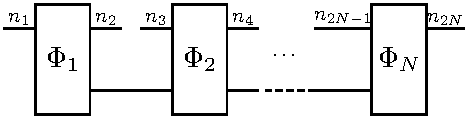
\includegraphics{general_comb.t1.pdf}
\end{center}


for some channels $\Phi_1,\dots, \Phi_N$.
{\color{red} Paviani, networks, etc}


\end{exm}


\begin{exm}[Partially classical maps]\label{exm:quantum_classical}  We may similarly define the basic
classical object as 
\[
\Pe_k:=(\mathbb R^k, \{x\in \mathbb R^k,\ \sum_i x_i=1\}).
\]
In this case, $\mathcal A_{\Pe_k}\cap \mathbb R^k_+$ is the probability simplex. We then
obtain further  useful objects by combining with the quantum objects. For example, it can be
easily seen that $\Se_n\multimap \Pe_k$ intersected with the cone $M_n^+\otimes \mathbb R^n_+$
corresponds to $k$-outcome {\em measurements}. Similarly, we obtain $k$-outcome {\em quantum instruments}
 from $\Se_m\multimap (\Se_n\otimes \Pe_k)$, {\em quantum multimeters} from $(\Se_m\otimes
\Pe_k)\multimap \Pe_l$, {\em quantum testers} from  $\Ce^N_{n_1,\dots,n_{2N}}\multimap
\Pe_k$, etc. 

\end{exm}




\subsection{First order and higher order objects}


We say that an object $X$ in $\Af$ is {\em first order} if $d_X=D_X-1$, equivalently, $S_X=V_X$.
Another equivalent condition is $d_{X^*}=0$, which means that $A_X$ is determined by a
single element $\tilde a_X\in V_X^*$ as 
\[
A_X=\{\tilde a_X\}^*,\qquad A^*_X=\{\tilde a_X\}.
\]
Note that first order objects, resp. their duals, are exactly those satisfying
condition (iii), resp. condition (ii), in Proposition \ref{prop:noncompact}, in
particular, $(X\otimes Y)^*=X^*\otimes Y^*$ for first order objects $X$ and $Y$.


{\em Higher order objects} in $\Af$ are objects  obtained from a finite set $\{X_1,\dots,X_n\}$ of first order objects by
taking tensor products and duals. The above is indeed a set, so that all the objects are
different (though they may be isomorphic) and the ordering is not essential. We will also
assume that the monoidal  unit $I$ is not contained in this set. By definition of
$X\multimap Y$,
and since we may identify $X\multimap I$ with $X^*$, we see that higher order objects are
also generated by applying the internal hom inductively on $\{X_1,\dots, X_n\}$ if we allow $X_i=I$ for some  
$i$. It follows that the objects introduced  in Examples \ref{exm:quantum_maps} and
\ref{exm:quantum_classical}
are indeed higher order objects in $\Af$  according to the above definition.


Of course, any first order
object is also higher order with $n=1$. Note that we cannot say that a higher order object
generated from $\{X_1,\dots, X_n\}$ is automatically ''of order $n$'', as the following lemma shows. 

\begin{lemma}\label{lemma:1ordertensor} Let $X$, $Y$ be first order, then $X\otimes Y$ is
first order as well.

\end{lemma}

\begin{proof} We have $S_{X\otimes Y}=S_X\otimes S_Y=V_X\otimes V_Y=V_{X\otimes Y}$.

\end{proof}

As we have seen, higher order objects are obtained by applying the internal hom
iteratively. The following properties of such iterations are easily seen from the
definition and properties of $\multimap$. 

\begin{lemma}\label{lemma:combs} Let $X,Y,Z$ be any objects in $\Af$. Then we have
\begin{enumerate}
\item[(i)] $Z\multimap (X\multimap Y)\simeq (Z\otimes X)\multimap Y\simeq X\multimap
(Z\multimap Y)$.
\item[(ii)] If $X=(V_X,\{\tilde a_X\}^*)$ and $Y=(V_Y, \{\tilde a_Y\}^*)$ are first order, 
then $Z\multimap (X\multimap Y)$ is determined as
\[
A_{Z\multimap (X\multimap Y)}=\{w\in V_{Z}^*\otimes V_X^*\otimes V_Y, (id\otimes \tilde a_Y)(w)\in
A_Z^*\otimes \tilde a_X\}.
\]

\end{enumerate}


\end{lemma}

Note also that since we identify $X^{**}=X$ for any object $X$, the isomorphisms in (i)
above are given by the symmetries in $\FV$, that is, by permutations of the components in
the tensor products of the underlying vector spaces. To save some parentheses, we also
assume that the internal homs associate to the right, so we write
$X\multimap Y\multimap Z$ instead of $X\multimap (Y\multimap Z)$. 

\begin{exm}[Channels and Combs] Let  $X$ and $Y$ be first order objects in $\Af$. As we
have seen, $C_1(X,Y):= X\multimap Y$ is then a higher order object, called a {\em channel} or {\em
1-comb} (We slightly  abuse
the terminology here).  We will inductively construct higher order objects in $\Af$,
similarly as in Example \ref{exm:quantum_maps}. An
{\em $N$-comb} over first order objects $X_1,\dots,X_{2N}$ is an object
\begin{align*}
C_N(X_1,\dots,X_{2N})&:=C_{N-1}(X_2,\dots,X_{2N-2})\multimap (X_1\multimap X_{2N})\\
&\simeq X_{1}\multimap C_{N-1}(X_2,\dots,X_{2N-2})\multimap X_{2N}\\
&\simeq X_1\multimap(X_2\multimap\dots \multimap (X_{N}\multimap
X_{N+1})\multimap \dots \multimap X_{2N-1})  \multimap X_{2N}
\end{align*}
where the isomorphisms follow by Lemma \ref{lemma:combs}. The subspace $A_{C_N}$ for an
$N$-comb $C_N$ can be found inductively, using Lemma \ref{lemma:combs} (ii).
If $X_1,\dots, X_{2N}$ are quantum objects, then $\tilde a_{X_i}$ is always a multiple of
the identity, so we obtain the characterization of quantum combs  in [paviani].



\end{exm}




\section{Combinatorial description of higher order objects}


{\em Types} of higher order quantum maps were introduced in [paviani],{\color{red}
something more here} who gave a combinatorial
description of the corresponding affine subspaces. More precisely, they show that the
affine subspace for the corresponding type of higher order objects can be combined from
some mutually independent {\color{red} linear subspaces}, and any such combination can be
labelled by a binary string.

In this section we show that we can have a similar description of higher order objects in
$\Af$, though the construction is slightly more complicated, because there is in general
no distinguished element in $A_X$ for a first order object $X$. We also use boolean
functions to characterize the  subsets of binary strings corresponding to the type, which will turn out useful for further description of
 types.  We will use the definitions, notations and results given in Appendix
\ref{sec:boolean}.

For a first order object $X=(V_X, \{\tilde a_X\}^*)$, let us pick an element $a_X\in
A_X$. We have a direct sum decomposition
\begin{equation}\label{eq:direct}
V_X=L_{X,0}\oplus L_{X,1},
\end{equation}
where $L_{X,0}:= \mathbb R\{a_X\}$, $L_{X,1}:=\{\tilde a_X\}^\perp=L_X$.
We define the {\em conjugate object}  as $\tilde X=(V_X^*,\{a_X\}^*)$. Note that we always
have $\tilde a_X\in A_{\tilde X}$ and with the choice $a_{\tilde X}=\tilde a_X$, we obtain 
$\tilde{\tilde X}=X$ and 
\begin{equation}\label{eq:complement}
L_{\tilde X,u}=L_{X,1-u}^\perp,\qquad u\in \{0,1\}.
\end{equation}
These  definitions depend on the choice of $a_X$, but we will assume below that this
choice is fixed and that we choose $a_{\tilde X}=\tilde a_X$. Since we will always work
with a finite set of objects at a time, this will not create any problems. 

 A  first order quantum
or classical object  is the set of states $\Se_n$ or the set of probability distributions
$\Pe_k$, see Examples \ref{exm:quantum_maps}, \ref{exm:quantum_classical}.
In these cases, $a_X$ will be chosen as the appropriate multiple of the identity.
 Note that for quantum objects we have
 \[
L_{X,0}=L_{\tilde X,0}= \mathbb R\{E_n\},\qquad  L_{X,1}=L_{\tilde X,1}= \{E_n\}^\perp
 \]
(similarly for classical objects). 


Let $X_1,\dots,X_n$ be first order objects in $\Af$. Let $a_{X_i}\in A_{X_i}$ be fixed and
let $\tilde X_i$ be the conjugate first order objects. Let us denote $V_i=V_{X_i}$ and 
\[
L_{i,u}:= L_{X_i,u},\qquad  \tilde L_{i,u}:= L_{\tilde X_i,u} \qquad u\in \{0,1\},\ i\in [n].
\]
For a string $s\in \{0,1\}^n$, we define
\[
L_s:=L_{1,s_1}\otimes\dots \otimes L_{n,s_n}, \qquad \tilde L_s:=\tilde
L_{1,s_1}\otimes\dots \otimes \tilde L_{n,s_n},
\]
then by \eqref{eq:direct} we have the direct sum decompositions 
\[
V:=V_1\otimes \dots \otimes V_n=\sum_{s\in \{0,1\}^n} L_s,\qquad V^*=V_1^*\otimes
\dots\otimes V_n^*=\sum_{s\in \{0,1\}^n} \tilde L_s
\]
(here $\sum$ denotes the direct sum).


\begin{lemma}\label{lemma:Lperp}   For any $s\in \{0,1\}^n$, we have 
\[
L_s^\perp=
\sum_{t\in\{0,1\}^n} (1-{\chi}_s(t))\tilde L_t,\qquad \tilde L_s^\perp=
\sum_{t\in\{0,1\}^n} (1-{\chi}_s(t))L_t.
\]
Here $\chi_s:\{0,1\}^n\to\{0,1\}$ is the characteristic function of $s$. 

\end{lemma}

\begin{proof} Using \eqref{eq:complement} and the direct sum decomposition of $V_i^*$, we get
\begin{align*}
\left(L_{1,s_{1}}\otimes \dots\otimes L_{n,s_{n}}\right)^\perp&= \bigvee_j\left(
V_{1}^*\otimes
\dots \otimes V_{j-1}^*\otimes \tilde L_{j,1-s_{j}}\otimes V_{j+1}^*\otimes\dots \otimes
V_{n}^*\right)\\
&= \bigvee_j \left( \sum_{\substack{t\in \{0,1\}^n\\ t_{j}\ne s_{j}}} \tilde
L_{1,t_{1}}\otimes\dots \otimes \tilde
L_{n,t_{n}}\right)\\
&= \sum_{\substack{t\in \{0,1\}^n\\ t\ne s}} \left( \tilde L_{1,t_{1}}\otimes\dots \otimes \tilde
L_{n,t_{n}}\right).
\end{align*}
The proof of the other equality is the same.

\end{proof}

For the fixed first order objects  $X_1,\dots,X_n$ and their conjugate objects $\tilde
X_1,\dots,\tilde X_n$, we introduce the following definitions. Put $a:= a_1\otimes\dots \otimes  a_n$, $\tilde a:= \tilde
a_1\otimes\dots\otimes  \tilde a_n$.
For  $f\in \Fe_n$ (see Appendix \ref{app:functions}) define 
\begin{equation}\label{eq:SfAf}
S_f=S_f(X_1,\dots,X_n):=\sum_{s\in \{0,1\}^n} f(s)L_s,\qquad
A_f=A_f(X_1,\dots,X_n):=S_f\cap \{\tilde a\}^*.
\end{equation}
It is clear from definition that $A_f$ is an affine subspace. Since
$f(\theta_n)=1$, the space $S_f$ always contains the subspace $L_0=L_{1,0}\otimes\dots\otimes
L_{n,0}=\mathbb R\{a\}$ and it is clear that $L_s\subseteq \{\tilde a\}^\perp$ for any
$s\ne \theta_n$. It follows that $a\in A_f$, so that $A_f\ne \emptyset$, and since $A_f\subseteq
\{\tilde a\}^*$, we see that  $A_f$ is proper and $\tilde
a\in A^*_f$.  It is easy to see that we have
\[
\lin(A_f)=\sum_{s\in\{0,1\}^n\setminus\{\theta_n\}} f(s)L_s,\qquad \Span(A_f)=S_f.
\]
We may now define the objects
\[
X_f=X_f(X_1,\dots, X_n):=(V,A_f(X_1,\dots,X_n))
\]
in $\Af$.

\begin{prop}\label{prop:Xf_const} Let $X_1,\dots,X_n$ be first order objects and $\tilde
X_1,\dots,\tilde X_n$ the conjugate objects. 
The map $\Fe_n\ni f\mapsto X_f(X_1,\dots,X_n)\in \Af$ is injective and we have the
following properties. 
\begin{enumerate}
\item[(i)] For the least and the largest element in $\Fe_n$, 
\[
X_{p_{n}}=\tilde X_1^*\otimes \dots\otimes \tilde X_n^*=(\tilde X_1\otimes \dots\otimes
\tilde X_n)^*,\qquad
X_{1_n}=X_1\otimes\dots\otimes X_n.
\]

\item[(ii)] The dual object satisfies
\[
X_f^*(X_1,\dots,X_n)=X_{f^*}(\tilde X_1,\dots,\tilde X_n).
\]
\item[(iii)] Let $f_1\in \Fe_{n_1}$, $f_2\in \Fe_{n_2}$. For the decomposition
$[n]=[n_1]\oplus[n_2]$,
\[
X_{f_1\otimes f_2}(X_1,\dots,X_n)=X_{f_1}(X_1,\dots, X_{n_1})\otimes
X_{f_2}(X_{n_1+1},\dots,X_n).
\]
\item[(iv)]  {\color{red} the symmetry $\sigma\in \permut_n$ defines an isomorphism} 
\[
X_f(X_{\sigma(1)},\dots,
X_{\sigma(n)})\xrightarrow{\sigma} X_{f\circ\sigma}(X_1,\dots,X_n).
\]
\end{enumerate}
\end{prop}

\begin{proof} Since  $L_s$, $s\in \{0,1\}$ is an independent decomposition of $V$, the
subspace $S_f$ has a unique decomposition in terms of $L_s$. It follows 
 that the map $f\mapsto A_f$, and hence also $f\mapsto X_f$ is injective. 
We have 
\[
S_{p_n}=L_{\theta_n}=\mathbb R\{a\}\qquad S_{1_n}=\sum_{s\in \{0,1\}^n}L_s=V,
\]
Since $X_1\otimes\dots\otimes X_n=(V,\{\tilde a\}^*)$ and $\tilde X_1\otimes \dots\otimes
\tilde X_n=(V^*,\{a\}^*)$, this proves (i). For (ii), it is enough to prove that 
$A^*_f(X_1,\dots,X_n)=A_{f^*}(\tilde X_1,\dots, \tilde X_n)$. To see this, we compute
using Lemma \ref{lemma:Lperp} and the fact that the subspaces form an independent
decomposition,
\begin{align*}
\Span( A^*_f)&=\lin(A_f)^\perp=\left(\sum_{s\in\{0,1\}^n\setminus\{0\}}
f(s)L_s\right)^\perp=
\bigwedge_{\substack{s\in\{0,1\}^n\\ s\ne 0, f(s)=1}}L_s^\perp=
\bigwedge_{\substack{s\in\{0,1\}^n\\ s\ne 0,
f(s)=1}}\left(\sum_{t\in\{0,1\}^n}(1-{\chi}_s(t))\tilde L_t\right)\\
&=\sum_{t\in\{0,1\}^n} \left(\bigwedge_{\substack{s\in \{0,1\}^n\\ s\ne 0, f(s)=1}}
(1-{\chi}_s(t))\tilde L_t\right)=\sum_{t\in \{0,1\}^n} f^*(t) \tilde L_t.
\end{align*}
To see the last equality, note that
\[
\bigwedge_{\substack{s\in \{0,1\}^n\\ s\ne 0, f(s)=1}}
(1-{\chi}_s(t))=\begin{dcases} 1 & \text{if } t=\theta_n\\ 1-f(t) & \text{if } t\ne \theta_n
\end{dcases} \ = f^*(t).
\]
The statement (iii) is easily seen from the definitions. To show (iv), compute
\begin{align*}
\sigma(S_f(X_{\sigma(1)},\dots,X_{\sigma(n)}))&=\sigma(\sum_{s} f(s)L_{\sigma(1),s_1}\otimes\dots \otimes
L_{\sigma(n),s_n})\\
&=\sum_s f(s) L_{1,s_{\sigma^{-1}(1)}}\otimes\dots\otimes
L_{n,s_{\sigma^{-1}(n)}}=S_{f\circ\sigma}(X_1,\dots,X_n).
\end{align*}
It folows that
\[
A_f(X_{\sigma(1)},\dots, X_{\sigma(n)})=S_f(X_{\sigma(1)},\dots, X_{\sigma(n)})\cap
\{\sigma^{-1}(\tilde a)\}^*=
\sigma^{-1}(A_{f\circ\sigma}(X_1,\dots,X_n)).
\]




\end{proof}


It follows from the independence of $L_s$, $s\in \{0,1\}^n$, that  the subspaces $S_f$ form a
distributive sublatice in the lattice of subspaces of $V$ and we clearly have 
$f\le g$ if and only if $S_f\subseteq S_g$, and $S_{f\wedge g}=S_f\cap S_g$, $S_{f\vee
g}=S_f\vee S_g$. For the affine subspaces, we get that similarly $f\le g$ iff
$A_f\subseteq A_g$ and  $A_{f\wedge g}=A_f\cap A_g$, $A_{f\vee g}=A_f\vee
A_g:=\aff(A_f\cup A_g)$. 
In terms of the objects in the category $\Af$, we get that $f\le g$ if and only if $X_f\xrightarrow{id_V} X_g$
(note that the identity of $V$ in $\FV$ is not necessarily a morphism in $\Af$). We also
remark that if $k\le f,g\le h$, then the following diagrams are  a pullback resp.  pushout:
\[
\xymatrix{
X_{f\wedge g}\ar[r]^{id_V}
\ar[d]_{id_V} & X_f\ar[d]^{id_V} \\
X_g \ar[r]_{id_V}& X_h
} \qquad 
\xymatrix{
X_{k}\ar[r]^{id_V}
\ar[d]_{id_V} & X_f\ar[d]^{id_V} \\
X_g \ar[r]_{id_V}& X_{f\vee g}
}
\]

We have also seen that $S_{f\otimes g}=S_f\otimes S_g$. It follows that the lattice structure of
$\Fe_n$, together with the operation $\otimes$, is reflected in the corresponding
subspaces of $V$. If all the objects are quantum (or classical), we have an identification
$V=V^*$, so that we have also the conjugation captured as $S_{f^*}=S_f^\perp + S_{p_n}$. 
In this way, $S_f$, $f\in \Fe_n$ becomes a boolean algebra endowed with a product
$\otimes$ {\color{red} see [hoffreumon]}. All these structures are inherited from $\Fe_n$.



Our main goal in this paragraph  is to show that the higher order objects are precisely those of the form
$Y=X_f(X_1,\dots,X_n)$ for some choice of the
first order objects $X_1,\dots, X_n$ and a function $f$ that belongs to a special subclass
 $\Te_n\subseteq \Fe_n$. The elements of this subclass will be called the {\em type
 functions},
 or {\em types}, and are defined as those functions in $\Fe_n$ that can be obtained by taking
 the constant function $1_1$ in each coordinate and then repeatedly applying duals and tensor
 products of such functions in any order. The set of indices for which the corresponding
 coordinate  was subjected to taking the dual an odd  number of times will be called the
{\em inputs} (of $f$) and denoted by $I=I_f$, indices  in $O=O_f:=[n]\setminus I_f$ will be
called {\em outputs}. The reason for this terminology will become clear later. It is easy to observe that if $f\in \Te_n$, then $O_{f^*}=I_f$ and $I_{f^*}=O_f$. Further,
for $f_1\in \Te_{n_1}$, $f_2\in \Te_{n_2}$, we have $O_{f_1\otimes f_2}=O_{f_1}\oplus
O_{f_2}$ and  $I_{f_1\otimes f_2}=I_{f_1}\oplus
I_{f_2}$, see \eqref{eq:disu} for the definition.

We have the following  description of the sets of type functions.

\begin{prop}\label{prop:type_min} The system  $\{\Te_n\}_{n\in \mathbb N}$ is the smallest
system of sets such that
\begin{enumerate}
\item $\Te_1=\Fe_1$, $\Te_n\subseteq \Fe_n$ for all $n$,

\item For $[n]=[n_1]\oplus [n_2]$, $\Te_{n_1}\otimes \Te_{n_2}\subseteq \Te_{n}$,
\item $\Te_n$  is invariant under permutations: if $f\in \Te_n$, then $f\circ \sigma\in
\Te_n$ for any $\sigma\in \permut_n$,
\item $\Te_n$  is invariant under complementation: if $f\in \Te_n$ then $f^*\in \Te_n$.

\end{enumerate}

\end{prop}


\begin{proof} It is clear by construction that any system of subsets $\{\Se_n\}_n$ with
these properties must contain the type functions and that $\{\Te_n\}_n$ itself has these
properties.

\end{proof}

  

Assume that  $Y$ is a higher order object constructed from a set of distinct first
order objects $Y_1,\dots, Y_n$, $Y_i=(V_{Y_i},\{\tilde a_{Y_i}\}^*)$.
%, we will write$Y\sim\{Y_1,\dots,Y_n\}$ in this case. 
Let us fix elements $a_{Y_i}\in A_{Y_i}$ and construct the conjugate objects $\tilde Y_i$. 
By compactness of $\FV$, we may assume (relabeling the objects if necessary) that the vector space of $Y$ has the form
\[
V_Y=V:=V_{1}\otimes \dots\otimes V_{n},
\]
where  $V_i$ is either $V_{Y_i}$ or $V_{Y_i}^*$, according to whether $Y_i$ was subjected
to taking duals an even or odd number of times. Similarly as for the type functions, the indices such that the first
case is true will be called the  outputs and the subset of outputs in $[n]$ will be denoted
by $O$, or $O_Y$, when we need to specify the object. The set $I=I_Y:=[n]\setminus O_Y$ is
the set of  inputs. Note that although we cannot yet exclude that $Y$ was constructed from
$Y_i$ in several different ways, the input and output spaces are always the same, fixed in 
the structure of $V$.

\begin{theorem}\label{thm:boolean} Let $Y$ be a higher order object, constructed from first
order objects $Y_1,\dots,Y_n$. For $i\in [n]$, let 
$X_i=Y_i$ if $i\in O_Y$ and $X_i=\tilde Y_i$ for $i\in I_Y$. 
There is a unique function $f\in \Te_n$, with $O_f=O_Y$,  such that 
\[
Y= X_f=(V, A_f(X_1,\dots,X_n)).
\]
Conversely, let $X_1,\dots, X_n$  be first order objects  and let
$f\in \Te_n$. Then $Y=X_f$ is a higher order object with $O_Y=O_f$, with underlying first
order objects $Y_1,\dots, Y_n$, where $Y_i=X_i$ for $i\in O_f$ and $Y_i=\tilde X_i$ for
$i\in I_f$.  

\end{theorem}

\begin{proof} Since the map $f\mapsto X_f$ is injective, uniqueness is clear.  To show existence of this
function, we will proceed by induction on $n$. For $n=1$, the assertion is easily seen
to be true, since in this case, we we have either $Y=Y_1$ or $Y=Y_1^*$. In the first case,
$O=\{1\}$, $I=\emptyset$, 
$X_1=Y_1$ and 
\[
S_Y=V_Y=V_1=L_{1,0}\oplus L_{1,1}=1(0)L_{1,0}\oplus 1(1)L_{1,1}=S_1(X_1),
\]
so in this case $f\in \Te_1$ is the constant 1. If $Y=Y_1^*$, we have $O=\emptyset$,
$I=\{1\}$, $X_1=\tilde
Y_1$, and then
\[
S_Y=\mathbb R\{\tilde a_{Y_1}\}=L_{1,0}=p_1(0)L_{1,0}\oplus p_1(1)L_{1,1}=S_{p_1}(X_1),
\]
so that $f=1^*=p_{1}\in \Te_1$. It is clear that $O_f=O_Y$ in both cases. 

Assume now that the assertion is true for
all $m<n$. By construction, $Y$ is either the tensor
product $Y=Z_1\otimes Z_2$, with
$Z_1$ constructed from $Y_{1},\dots, Y_{m}$ and $Z_2$ from $Y_{{m+1}},\dots,
Y_{n}$,
 or $Y$ is the dual of such a product. Let us assume the first case. It is clear that
 $O_{Z_1}\oplus O_{Z_2}=O_Y$, and similarly for $I$, so that the corresponding objects
 $X_1,\dots, X_m$ and $X_{m+1},\dots,X_n$  remain the same. By the induction 
assumption, there are functions $f_1\in \Te_m$ and $f_2\in \Te_{n-m}$ such that
$O_{f_1}=O_{Z_1}$, $O_{f_2}=O_{Z_2}$ and,  by Proposition \ref{prop:Xf_const}(iii), 
\[
Y=Z_1\otimes Z_2=X_{f_1}(X_1,\dots,X_m)\otimes X_{f_2}(X_{m+1},\dots,X_n)=X_{f_1\otimes
f_2}(X_1,\dots,X_n)
\]
This implies the assertion, with $f=f_1\otimes f_2\in \Te_n$ and $O_f=O_{f_1}\oplus
O_{f_2}=O_Y$. 
To finish the proof, it is now enough to observe that if the assertion holds for $Y$ then
it also  holds for $Y^*$. So assume that $Y=X_f(X_1,\dots,X_n)$ for some $f\in \Te_n$, 
then by Proposition \ref{prop:Xf_const}(ii), $Y^*=X_f^*=\tilde X_{f^*}(\tilde X_1,\dots,\tilde X_n)$. 
By the construction of conjugate objects, we have  $\tilde X_i=\tilde{\tilde Y}_i=Y_i$
if $i\in I_{Y}$ and $\tilde X_i=\tilde {Y}_i$ if $i\in O_Y$. Since by definition and the
assumption,
$O_{Y^*}=I_Y=I_f=O_{f^*}$, this proves the statement.

The converse is proved by a similar induction argument, using Proposition
\ref{prop:Xf_const}.

\end{proof}

Let us stress that in general, the objects $X_f$ depend on the choice of the elements
$a_{X_i}$. From the above proof, it is clear that  the  description in Theorem
\ref{thm:boolean} does not depend on the choice of the elements $a_{Y_i}\in A_{Y_i}$.
Furthermore, if all the first order objects are quantum, we have
$S_f(X_1,\dots,X_n)=S_f(\tilde X_1,\dots,\tilde X_n)$ and both $a$ and $\tilde a$ are 
some, possibly different,  multiples of the identity. The spaces $A_f(X_1,\dots,X_n)$ and $A_f(\tilde X_1,\dots,\tilde
X_n)$ differ only by this multiple. 

%\subsection{Type funtions and higher order objects}
%
%
%Let $\Te_n\subseteq \Fe_n$ be defined as the subset generated from the constant 
%function $1$ on $\{0,1\}$ by taking duals and tensor products. For example, we have
%\[
%\Te_1=\Fe_1=\{1,1^*\},\quad
%\Te_2=\{1\otimes 1, (1\otimes 1)^*, 1\otimes 1^*,1^*\otimes 1, (1^*\otimes 1)^*,
%(1\otimes 1^*)^*\},
%\]
%etc.  Elements of $\Te_n$ will be called {\em type functions}. Similarly as for the higher order
%objects, the indices in $[n]$ such that the corresponding
%component was subjected to taking the dual an even number of times will be called the
%outputs (of $f$) and denoted by $O=O_f$, indexes in $I=I_f:=[n]\setminus O_f$ will be
%called inputs. From the proof of Proposition \ref{prop:boolean}, it is easily seen that a
%higher order object is of the form $Y=X_f$ for a function $f\in \Te_n$ with the same outputs (and of
%course also inputs) as $Y$. We next show that the converse is true. 
%
%
%\begin{prop}\label{prop:type_hom}
%\end{prop}
%
%\begin{proof} As before, we will proceed by induction on $n$. For $n=1$, we only have the
%possibilities $f=1$ or $f=1^*$. In the first case, $O=[1]$ and we get
%\[
%S_f=1L_{1,0}\oplus 1L_{1,1}= V_{1},
%\]
%so that $X_f=(V_1,\{\tilde a_1\}^\sim)=X_1$. In the second case, $O=\emptyset$ and 
%\[
%S_f=1L_{1,0}=\mathbb R\{a_1\},
%\]
%so that $X_f=(V_1,\{a_1\})=\tilde X_1^*$. Assume next that the statement
%is true for all $m<n$ and assume that $f=f_1\otimes f_2$ for some $f_1\in \Fe_m$, $f_2\in
%\Fe_{n-m}$, then it is easily seen that $Y=Z_1\otimes Z_2$ for $Z_1=X_{f_1}(X_1,\dots,X_m)$ and
%$Z_2=X_{f_2}(X_{m+1},\dots,X_n)$. 
%By the induction assumption, $Z_1$ and $Z_2$ are higher order objects, with
%$O_{Z_i}=O_{f_i}$, it follows that $Y$ is a higher order object with $O_Y=O_{Z_1}\cup
%O_{Z_2}=O_{f_1}\cup O_{f_2}=O_f$.
%
%Finally, assume that the statement is true for $f\in \Fe_n$, we will show that it holds
%for $f^*$. By  Lemma \ref{lemma:Xf}, we see that $X_{f^*}(X_1,\dots,X_n)=X^*_f(\tilde
%X_1,\dots,\tilde X_n)$. By the assumption, $X_f$ is a higher order object with underlying
%first order objects $\tilde X_i$ for $i\in O_f$ and $\tilde{\tilde X}_i$ for $i\in I_f$. 
%Since $O_{f^*}=I_f$, the statement follows.
%
%
%
%\end{proof}
%

\section{The type functions}

The aim of this section is to gain some understanding into the structure and properties of
the set of type functions. We start by an important example.


\begin{exm}\label{exm:type_channels}
Let $T\subseteq [n]$. It is easily seen that the function  $p_T$ (see Example \ref{ex:pS}
in Appendix \ref{sec:boolean}) is a type function, since we have
\[
p_T(s)=\Pi_{j\in T}(1-s_j)=\Pi_{j\in T} 1^*(s_j)=(\otimes_{j\in T}1^*)(s).
\]
By definition, $T$ is the set of inputs for $p_T$. Let $X_1,\dots, X_n$ be 
 first order objects. Let $k=|T|$ and let $\sigma\in \permut_n$ be such that
$\sigma^{-1}(T)=[k]$. Then 
$p_T\circ \sigma=p_{k}\otimes 1_{n-k}$. By Proposition \ref{prop:Xf_const}, it follows that
we have the {\color{red} isomorphism}  
\[
X_{p_T}(X_1,\dots,X_n)\overset{\sigma}{\simeq}X_{p_{k}\otimes 1_{n-k}}(X_{\sigma^{-1}(1)},\dots, X_{\sigma^{-1}(n)})=\tilde
X_T^*\otimes X_{[n]\setminus T},
\]
here $\tilde X_T=\otimes_{j\in T} \tilde X_j$ and $X_{[n]\setminus T}=\otimes_{j\in
[n]\setminus T} X_j$ are first order object by Lemma \ref{lemma:1ordertensor}.
It follows that $p_T$ describes replacement channels with set of input indices  $T$. By duality,
we obtain the isomorphisms
\[
X_{p_T^*}(X_1,\dots,X_n)=X_{p_T}^*(\tilde X_1,\dots,\tilde X_n)\overset{\sigma}{\simeq} (X_T^*\otimes \tilde
X_{[n]\setminus T})^*\simeq  \tilde X_{[n]\setminus T}\multimap X_T,
\]
where $\rho$ is the transposition in $\permut_2$. It follows
that $p^*_T=1-p_T+p_{n}$ corresponds to all channels with output indices $T$.

\end{exm}


\begin{lemma}\label{lemma:fh_setting} Let $f\in\Te_n$ and let $O_f=O$,  $I=I_f$. Then
\[
p_I\le f\le p_O^*.
\]

\end{lemma}

\begin{proof} This is obviously true for $n=1$. Indeed, in this case,
$\Te_1=\Fe_1=\{1_1=p_\emptyset,1_1^*=p_{1}\}$. If $f=1_1$, then $O=[1]$, $I=\emptyset$ and 
\[
p_I=p_{\emptyset}=1_1=p_O^*,
\]
the case  $f=p_1$ is obtained by taking complements. Assume that the assertion holds for
$m<n$. Let $f\in \Te_n$ and assume that  $f=g\otimes h$ for some  $g\in
\Te_m$, $h\in \Te_{n-m}$.  By the assumption,
\[
p_{I_g}\otimes p_{I_h}\le g\otimes h\le p^*_{O_g}\otimes p^*_{O_h}\le (p_{O_g}\otimes
p_{O_h})^*,
\]
the last inequality follows from Lemma \ref{lemma:fproduct}. With the decomposition
$[n]=[m][m+1,n]$, we have   
$O_f=O_g\oplus O_h$, $I_f=I_g\oplus I_h$, so that by Lemma \ref{lemma:PSPT}, 
$p_{O_f}=p_{O_g}\otimes p_{O_h}$ and
similarly for $p_{I_f}$. Now notice that for any $f\in \Te_n$ we have either $f\approx g\otimes
h$ or $f\approx (g\otimes h)^*$. Since the inequality is easily seen to be preserved by
permutations, and reversed by duality which also swiches the input and output sets, the
assertion is proved.

\end{proof}


Combining this with Proposition \ref{prop:Xf_const}, we get the following result
(cf. cite). 

\begin{coro}\label{coro:setting} Let $Y$ be a higher order objects constructed from
first order objects $Y_1,\dots, Y_n$,  $O_Y=O$,
$I_Y=I$.  Then there are
$\sigma_1,\sigma_2\in \permut_n$ such that we have the  morphisms 
\[
Y_I^*\otimes Y_O\xrightarrow{\sigma_1} Y
\xrightarrow{\sigma_2} [Y_I, Y_O].
\]
 


\end{coro}



We also obtain  a simple  way to identify the output indices  of a type
function.

\begin{prop}\label{prop:fh_outputs} For $f\in \Te_n$, $j\in O_f$ if and only if
$f(e^j)=1$, here $e^j=\delta_{1,j}\dots\delta_{n,j}$.


\end{prop}


\begin{proof} Let $i\in O_f$, then by Lemma \ref{lemma:fh_setting}, $p_{I_f}(e^i)=1\le
f(e^i)$, so that $f(e^i)=1$. Conversely, if $f(e^i)=1$, then by the other inequality in
lemma \ref{lemma:fh_setting}, $p_{O_f}(e^i)=0$, whence $i\in O_f$.


\end{proof}


\begin{exm}\label{exm:T2} The type functions for $n=2$ are given as (writing $\bar u=1-u$
for $u\in \{0,1\}$, and $s=s_1s_2$):
\[
1_2(s)=1,\quad p_{2}(s)=\bar s_1\bar s_2,\quad p_{[1]}(s)=\bar s_1, \quad 
p_{[1]}^*(s)= 1-\bar s_1+\bar
s_1\bar s_2,
\]
and functions  obtained from these by permutation, which gives 6 different elements.
We have seen in Appendix \ref{app:functions} that  $\Fe_n$ has $2^{2^n-1}$ elements, so that $\Fe_2$ has 8
elements in total. The two remaining functions  are
\[
g(s)=1-\bar s_1-\bar s_2+2\bar s_1s_2,\qquad g^*(s)=\bar s_1+\bar s_2-\bar s_1\bar s_2.
\]
It can be  checked directly from Lemma \ref{lemma:fh_setting} and
Proposition \ref{prop:fh_outputs} that $g$ is not a type function. Indeed, if $g\in \Te_2$, we would have $O_g=\emptyset$, so that
$p_{2}\le g\le p_\emptyset^*=p_{2}$, which is obviously not the case. Clearly, also the
complement $g^*\notin \Te_2$. Notice also that $g^*=p_{[1]}\vee p_{[2]}$, so that
$\Te_2$ is not a lattice. 

\end{exm}


Since $\Fe_2$ can be identified as a sublattice in $\Fe_n$ for
all $n\ge 2$ as $\Fe_2\ni f\mapsto f\otimes 1_{n-2}\in \Fe_n$, the above example shows
that  $\Te_n$, $n\ge 2$ is a  subposet in the distributive lattice 
$\Fe_n$ but itself not a lattice,  so that for $f_1,f_2\in
\Te_n$, none of $f_1\wedge f_2$ or $f_1\vee f_2$ has to be a type function.
Nevertheless, we have by the above results that all type functions with the same output
indices are contained in the interval $p_I\le f\le p_O^*$, which is a distributive
lattice. Elements of such an interval  will be called {\em subtypes}. It is easily seen
that for $n=2$ all subtypes are type functions, but it is not difficult to find a subtype
for $n=3$ which is not in $\Te_3$. The objects corresponding to
subtypes are not necessarily
higher order objects, but are embedded in  $[Y_I,Y_O]$ and contain the replacement
channels. If $f_1$ and $f_2$ have the same output set, then  $f_1\vee f_2$ and $f_1\wedge
f_2$ are subtypes. {By the remarks below Proposition \ref{prop:Xf_const}, the corresponding objects can be
obtained by pushouts resp. pullbacks of the higher order objects corresponding to $f_1$
and $f_2$.}




\subsection{The poset $\Pe_f$}



%Here we introduce the basic tools for describing and visualising the structure of type
%functions. We will need the notions and results of Appendix \ref{app:functions, posets}.


By Theorem \ref{thm:mobius}, any boolean function has a unique expression of the form
\[
f=\sum_{T\subseteq [n]} \hat f_Tp_T,
\]
where $\hat f$ is the M\"obius transform of $f$. Using this, we introduce a poset related
to $f$, which will be useful for description of the structure of $f$. We will need the
definitions and basic results in Appendix \ref{app:poset}.

Let $\mathcal P_f$ be the subposet in the
distributive lattice $2^n$,  of elements such that
$\hat f_T\ne 0$. The main result of this paragraph is that any type function $f\in \Te_n$ is fully determined by $\Pe_f$.  
We first need to show how some of the operations on type functions are reflected on  $\Pe_f$.

\begin{lemma}\label{lemma:Pf} Let $f\in \Te_n$.
\begin{enumerate}

\item[(i)] If $\sigma\in \permut_n$, then $S\mapsto \sigma^{-1}(S)$ is an isomorphism of
$\Pe_{f}$ onto $\Pe_{f\circ\sigma}$.
\item[(ii)] For $g\in \Te_m$ and the decomposition $[n+m]=[n]\oplus [m]$, we have
$\Pe_{f\otimes g}\simeq \Pe_{f}\times \Pe_g$, with the isomorphism given by $(S,T)\mapsto
S\oplus T$ and 
\[
(\widehat{f\otimes g})_{(S,T)} =\hat f_S\hat g_T.
\]

\end{enumerate}


\end{lemma}

\begin{proof} The statement is proved using Lemma \ref{lemma:PSPT}.  We have
\[
f\circ \sigma=\sum_{S\subseteq [n]} \hat f_S p_S\circ\sigma=\sum_{S\subseteq [n]} \hat
f_Sp_{\sigma^{-1}(S)}=\sum_{S\subseteq [n]} \hat
f_{\sigma(S)}p_{S}.
\]
The statement (i) now follows by uniqueness of the M\"obius transform. Similarly, for
$s=s^1s^2$,
\begin{align*}
f\otimes g(s)&=f(s^1)g(s^2)=\sum_{S\subseteq [n]}\sum_{T\subseteq [m]} \hat f_S\hat
g_Tp_S(s^1)p_T(s^2)=\sum_{S\subseteq [n]}\sum_{T\subseteq [m]} \hat f_S\hat
g_T(p_S\otimes p_T)(s)\\
&= \sum_{S\subseteq [n]}\sum_{T\subseteq [m]} \hat f_S\hat
g_T(p_{S\oplus T})(s).
\end{align*}
This proves (ii).





\end{proof}



\begin{theorem}\label{thm:graded} Let $f\in \Te_n$, then $\mathcal P_f$ is a graded poset
with even rank $r(f):=r(\Pe_f)\le n$.  Moreover, we have
\[
f=\sum_{S\in \mathcal P_f}(-1)^{\rho_f(S)}p_S,
\]
where $\rho_f$ is the rank function of $\Pe_f$.

\end{theorem}


\begin{proof} We will proceed by induction on $n$. Assume that  $n=1$. Then  $2^n=\{\emptyset, [1]\}$ and
$\Te_1=\{1_1,p_1\}$. For both type functions, $\mathcal P_f$ is a singleton, which 
is clearly a graded poset, with rank $k=0$ and trivial rank function $\rho_f\equiv 0$.  We have
\[
1_1=p_\emptyset=(-1)^{\rho(\emptyset)}p_\emptyset.
\]
The statement for $f=p_1$ follows by duality.  

Assume next that the statement holds for all $m<n$ and let $f\in \Te_n$. By construction,
it is enough to show that the property is invariant under permutations and complement and
that it holds for any $f$ of the form 
$f=f_1\otimes f_2$ for  type functions $f_1\in \Te_{n_1}$, $f_2\in \Te_{n_2}$.
So assume $f$ has the desired property and let $\sigma\in \permut_n$. 
It is clear by the
isomorphism in Lemma \ref{lemma:Pf} (i) that $\Pe_{f\circ\sigma}$ is a graded poset as
well, with the same even rank as $f$ and rank function
$\rho_{f\circ\sigma}=\rho_f\circ \sigma$. Then
\[
f\circ \sigma=\sum_{S\subseteq [n]} (-1)^{\rho_f(S)}p_S\circ\sigma=\sum_{S\subseteq [n]}
(-1)^{\rho_f\circ \sigma(S)}p_S.
\]
Further, assume that we have
\begin{align}
f^*&=1-f+p_n=(1-\hat f_\emptyset)p_\emptyset -
\sum_{\emptyset, [n]\ne S\subseteq [n]} \hat f_Sp_S+(1-\hat f_{[n]})p_n\notag\\
&=(1-\hat f_\emptyset)1 -\sum_{\substack{S\in \mathcal P_f\\ \emptyset \ne S,
[n]\ne S}}
(-1)^{\rho_f(S)}p_S+(1- \hat f_{[n]})p_n.\label{eq:dual_rank}
\end{align}
If $\emptyset \in \Pe_f$, then $\emptyset$ is the least element of $\Pe_f$, so that 
$\rho_f(\emptyset)=0$ and therefore $\hat f_\emptyset =
(-1)^0=1$. Similarly, if $[n]\in \Pe_f$, then $[n]$ is the largest element in $\Pe_f$,
hence it is the last element in any maximal chain. It follows that $\rho_f([n])=r(f)$ and hence
$\hat f_{[n]}=(-1)^{r(f)}=1$ (since the rank $r(f)$  is even). 
Therefore the equality \eqref{eq:dual_rank} implies that $\mathcal P_{f^*}$ differs from $\mathcal P_f$ only in the bottom  and
top elements:  $\emptyset \in \mathcal P_f$ iff  $\emptyset \notin \mathcal P_{f^*}$
and $[n] \in \mathcal P_f$ iff  $[n] \notin \mathcal P_{f^*}$. It follows that $\mathcal
P_{f^*}$ is graded as well, with rank  equal to $r(f)-2$, $r(f)$ or $r(f)+2$, which in any case
is even. Furthermore,  this also implies 
that for all $S\in \Pe_f$, $S\notin \{\emptyset, [n]\}$, we
have  $\rho_{f^*}(S)=\rho_f(S)\pm 1$, according to whether $\emptyset$ was added or removed. The
statement now follows from \eqref{eq:dual_rank}. 


Now assume that $f=f_1\otimes f_2$. By the induction assumption, both $\Pe_{f_1}$ and $\Pe_{f_2}$ are graded posets. By Lemma
\ref{lemma:Pf}, $\Pe_f\simeq \Pe_{f_1}\times \Pe_{f_2}$, so that $\Pe_f$  is a graded poset as well, with 
rank function $\rho_f(S,T)=\rho_{f_1}(S)+\rho_{f_2}(T)$ and rank $r(f)=r(f_1)+r(f_2)$.
 By Lemma \ref{lemma:Pf} (ii), we get 
\[
f=\sum_{S\subseteq [n_1], T\subseteq [n_2]} (\widehat {f_1})_S(\widehat
{f_2})_T p_S\otimes p_T=
\sum_{S\subseteq [n_1], T\subseteq [n_2]}(-1)^{\rho_{f_1}(S)+\rho_{f_2}(T)}p_{S\oplus T}.
\]
This finishes the proof.

\end{proof}


\begin{remark}\label{remark:n} Notice that we need to assume $n$ to be known. Indeed, for any $m$ and
$f$, $\Pe_f$ and $\Pe_{f\otimes 1_m}$ are the same, but the  two type functions are
different. In particular, the corresponding constructions of higher order
objects are different.

\end{remark}

In the course of the above proof, we have also shown the following.

\begin{coro}\label{coro:pf_dual} Let $f\in \Te_n$. Then $\Pe_{f^*}\setminus
\{\emptyset,[n]\}=\Pe_{f}\setminus
\{\emptyset,[n]\}$ and $\emptyset \in \Pe_f$ if and only if $\emptyset \notin \Pe_{f^*}$.
The same holds for $[n]$.

\end{coro}

\subsection{Labelled Hasse diagrams}

We  introduce {\em labels} for the elements of $\Pe_f$ in the following way. 
 For  $S\in \Pe_f$, put
\[
L_S:=\{i\in [n]\ : \ i\in S,\ \forall S'\subsetneq S, i\notin S'\}.
\]
In other words, $i$ is a label for $S$ if $S$ is a minimal element in the subposet of
elements containing $i$ in  $\Pe_f$. 
We will use the notation $L_{S,f}$ if the function $f$ has to be
specified. It is easily seen that for $S\in \mathrm{Min}(\Pe_f)$, $L_S=S$ and for any
$S\in \Pe_f$,  $S=\cup_{S'\subseteq S} L_{S'}$.
It follows that $f\in \Te_n$ (with known $n$) is fully determined by the order relation on $\Pe_f$ and the
label sets. All the information about $f$ can be therefore obtained from the {\em labelled
Hasse diagram} of $\Pe_f$. 

We next give some examples of simple type functions and their corresponding Hasse
diagrams. For this, we introduce the following notations: for $n\in \mathbb N$, put
\begin{equation}\label{eq:gammas}
\gamma_n:= \begin{dcases} \sum_{j=0}^n (-1)^jp_{[j]}, & \text{if $n$ is even}\\
\sum_{j=1}^n (-1)^{j-1}p_{[j]} & \text{if $n$ is odd}
\end{dcases}
\end{equation}
{\color{red} (recall that $[0]=\emptyset$)}. For each $n$, the poset $\Pe_{\gamma_n}$ is a chain of even
length and we will see in Section  \ref{sec:chains} below that $\gamma_n\in \Te_n$. 

\begin{exm} \label{exm:T2hasse} The labelled Hasse diagrams of elements in $\Te_2$
described in Example \ref{exm:T2} are up
to permuations as
follows:
\begin{center}
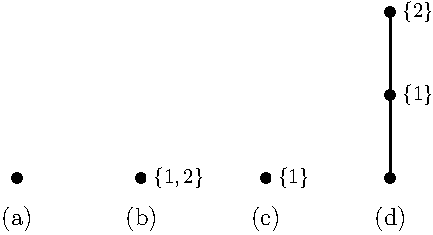
\includegraphics[scale=0.8]{t2_hasse.pdf}
\end{center}

Note that the diagram in (d) corresponds to the function $\gamma_2$.


\end{exm}

\begin{exm}\label{exm:T3}
As we can see above, for all elements in $\Te_2$, the corresponding
posets are chains. This is also true for $n=3$. Indeed, up to a permutation that does not change the chain structure, 
any $f\in \Te_3$ is either a product of two elements $g\in \Te_2$ and $h\in \Te_1$,
or the dual of such a  product. Since $g$ must be a chain and $|\Pe_h|=1$, their product
must be a chain as well. Taking the dual of a chain only adds/removes the least/largest
elements, so the dual of a chain must be a chain as well. All the functions depicted in
(a)-(d) above  are also contained in $\Te_3$. The only other
elements are (up to permutations):
\begin{center}
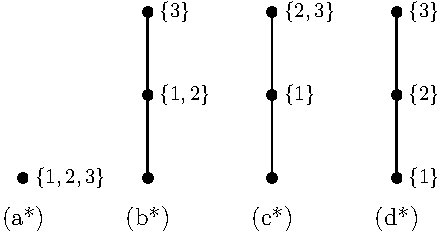
\includegraphics[scale=0.8]{t3_hasse.pdf}
\end{center}
Notice that in $\Te_3$, the function with diagram in (a*) is the conjugate of  the
function with diagram in  (a), etc. The diagram in (d*) correpsonds to $\gamma_3$.



\end{exm}


\begin{exm}\label{exm:T4} The only elements in $\Te_4$ such that the posets are not
isomorphic to any of the above have the diagrams:
\begin{center}
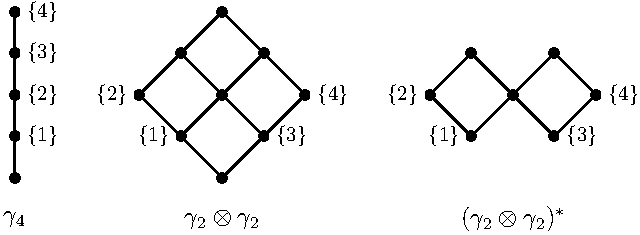
\includegraphics[scale=0.8]{t4_hasse.pdf}
\end{center}
\end{exm}

\medskip
Let us denote
\[
I_f^F:=\cap_{S\in \mathrm{Min}(\Pe_f)} L_S, \qquad O_f^F:=[n]\setminus
\cup_{S\in \Pe_f}L_S.
\]
It is easily checked by Proposition \ref{prop:fh_outputs} that any  $i\in O_f^F$ is an
output index, since in this case  we have
$f(e^i)=f(\theta_n)=1$. Such elements will be called
the {\em free outputs} of $f$. If $f$ has some free outputs, then necessarily $[n]\notin
\Pe_f$. Similarly, any  $j\in I_f^F$ is an input of $f$, since $j$ must be
contained in any $T\in \Pe_f$, so that $p_T(e^j)=0$ for all $T\in \Pe_f$ and consequently
$f(e^j)=0$. Such elements will be called {\em free
inputs} of $f$. The elements of $I_f^F\cup O_f^F$ will be called {\em free indices} of
$f$.  It is clear that $f\approx p_k\otimes g\otimes
1_l$, where
$k=|I_f^F|$, $l=|O_f^F|$  and $g\in \Te_{n-k-l}$ has no free indices. As posets,
$\Pe_f\simeq \Pe_g$,  with labels
\[
L_{S,f}=\begin{dcases} \sigma(L_{S,g}), &\text{if } S\notin \mathrm{Min}(\Pe_f)\\
\sigma(L_{S,g})\cup I^F_f, &\text {otherwise},
\end{dcases}
\]
for some $\sigma\in \permut_n$. Clearly, $n-k-l$ has to be specified for $g$. 



The  two distinguished elements $\emptyset$ and $[n]$, if present in $\Pe_f$, can be easily recognized
from its structure as a labelled poset. Indeed, $\emptyset\in \Pe_f$ if and only if
$\Pe_f$ has the  smallest element and it  has an empty label. 
Similarly, $[n]\in \Pe_f$ if and
only if $\Pe_f$ has  the largest element and $\cup_{S\in \Pe_f}L_S=[n]$. The basic operations on
type functions are obtained as follows. 

\begin{coro}\label{coro:Pf} Let $f\in \Te_n$, $g\in \Te_m$. Then
\begin{enumerate}
\item[(i)] For $\sigma\in \permut_n$,  $\Pe_{f\circ\sigma}\simeq \Pe_f$, with the labels
changed as $L_S\mapsto \sigma^{-1}(L_S)$.

\item[(ii)] $\Pe_{f^*}$ is obtained from from $\Pe_f$ by adding/removing $\emptyset$ and
$[n]$. If $[n]$ is added, then  $L_{[n],f^*}=O_f^F$.  All other elements and labels remain the same. 
\item[(iii)] Assume the decomposition $[n+m]=[n]\oplus[m]$. Then 
$\Pe_{f\otimes g}\simeq \Pe_f\times \Pe_g$, with label sets
\[
L_{(S,T)}=\begin{dcases} L_S\cup (n+L_T), & \text{if } S\in \mathrm{Min}(\Pe_f),\ T\in
\mathrm{Min}(\Pe_g)\\
L_S, & \text{if } S\notin \mathrm{Min}(\Pe_f),\ T\in
\mathrm{Min}(\Pe_g)\\
n+ L_T, &\text{if }S \in \mathrm{Min}(\Pe_f),\ T\notin
\mathrm{Min}(\Pe_g)\\
\emptyset, & \text{otherwise}.
\end{dcases}
\]



\end{enumerate}


\end{coro}


\begin{proof} We only need to prove the statements on the label sets. This is quite clear
in (i). In
(ii), if $[n]\in \Pe_{f^*}$, then the only new indices  not apearing below $[n]$ can be
the free outputs of $f$. In (iii), assume that $i\in L_{(S,T)}$, then $S\oplus T$ must be a minimal
element in $\Pe_{f\otimes g}$ containing $i$. Hence, either $i\in S$ or $i\in n+T$. In the
first case, $i\in (S'\oplus T')\le (S\oplus T)$ whenever  $i\in S'\le S$ and $T'\le T$, so we must have 
$i\in L_S$ and $T\in \mathrm{Min}(\Pe_g)$. Similarly, for $i\in n+T$, we get $i\in n+L_T$
and $S\in \mathrm{Min}(\Pe_f)$. 


\end{proof}



We next show that the input and output sets of $f\in \Te_n$ can be easily recognized from
the labels in $\Pe_f$. 

\begin{prop}\label{prop:pfinput} Let $f\in \Te_n$ and $i\in [n]$. Then
\begin{enumerate}
\item[(i)] All $S\in \Pe_f$ such that $i\in L_S$  have the same rank,  which will be
denoted by $r_f(i)$. If  $i\in O_f^F$,   we put $r_f(i):=r(f)+1$. 
\item [(ii)] $i\in O_f$ if and only if $r_f(i)$ is odd.

\end{enumerate}
\end{prop}



\begin{proof} As before, we proceed by induction on $n$. Both assertions are quite trivial for $n=1$,
so assume the statements hold for $m<n$. It is easily seen that the properties are
invariant under permutations. Assume (i) and (ii) hold for $f\in \Te_n$ and consider
$f^*$. If $i\in L_{[n],f^*}$, then $i$ cannot be contained in the label set of any other
element, so (i) is true. Also, by Corollary \ref{coro:Pf}, $L_{[n],f^*}=O_f^F$, so that
$i$ is an input of $f$. Since $[n]$ is the largest element of $\Pe_f$, 
$\rho_f([n])=r(f)$ is even, so that (ii) holds as well. By duality, both statements hold
if $i\in O_f^F$. In all other cases, $i\in L_{S,f}$ if and only if $i\in L_{S,f^*}$, so
(i) is true for $f^*$. By the
proof of Proposition \ref{thm:graded} we have  
$\rho_{f^*}(S)=\rho_f(S)\pm 1$ for any $S$, depending only on the fact whether $\emptyset
\in \Pe_f$. This implies that (i) and (ii)  are preserved by complementation.

 It is now enough to assume that
$f=g\otimes h$ for some $g\in \Te_m$ and $h\in \Te_{n-m}$. 
Suppose without loss of generality that $i\in [m]$, then $i\in L_{S\oplus T, f}$ if and
only if $i\in L_{S,g}$ and $T\in \mathrm{Min}(h)$.  Since then $\rho_h(T)=0$, we have
by the induction assumption
\[
\rho_f(S\oplus T)=\rho_g(S)+\rho_h(T)=\rho_g(S)= r_g(i).
\]
The statement (ii) follows from the fact that $i\in O_f$ if and only if $i\in O_g$.


\end{proof}


\subsection{Chains and combs}

 We have seen that for some type functions the poset $\Pe_f$ is a chain, which is also a
 basic example of a graded poset. A chain in $2^n$ has the form  $\Ce=\{S_1\subsetneq S_2\subsetneq \dots \subsetneq
S_N\}$, $S_i\subseteq [n]$. Note that the length of the chain $\Ce$ is $N-1$.
It is clear that  $\Ce$ is graded with rank $N-1$
and rank function $\rho(S_i)=i-1$. 

\begin{prop}\label{prop:chains} For a chain   $\Ce=\{S_1\subsetneq S_2\subsetneq \dots \subsetneq
S_N\}$, the function  
\[
f=f_\Ce:=\sum_{i=1}^N (-1)^{i-1} p_{S_i}
\]
is a type function if and only if $N$ odd. In this case, we say that $f$ is a chain type.

\end{prop}

\begin{proof}
By Proposition \ref{thm:graded}, if $f\in \Te_n$, then the rank of $f$ must be even, so
that $N$ must be odd. 
We will show that the converse is true. We proceed by induction on $N$. For $N=1$, we have
$f=p_{S_1}\in \Te_n$. Assume that the statement holds for all odd numbers $M<N$ and let
$\Ce$ be a chain as above. It is easily checked that   
\[
f\approx  p_{n_1}\otimes g\otimes 1_{n-n_N},
\]
where $n_i:=|S_i|$ and  $g\in
\Fe_{n_N-n_1}$ is the function for a chain $\Ce'$  in $2^{n_N-n_1}$ of the form $\Ce':=\{\emptyset\subsetneq S'_2\subsetneq \dots
\subsetneq [n_N-n_1]\}$. Since $f$ is a type function if $g$ is, this shows that we may assume that 
the chain $\Ce$ contains $\emptyset$ and $[n]$.  But then 
\[
f=1+\sum_{j=2}^{N-1} (-1)^{j-1}p_{S_j}+ p_{n} 
\]
and
\[
f^*=1-f+p_{n}=\sum_{j=1}^{N-2} (-1)^{j-1}p_{S_{j+1}},
\]
By the induction assumption $f^*\in \Te_n$, hence also $f=f^{**}\in
\Te_n$.
\end{proof}


Let $f\in \Te_n$ be a chain type and let $\Pe_f=\{S_1\subsetneq \dots \subsetneq
S_N\}$ be the corresponding chain. There is a decomposition of $[n]$ given as
\[
T_0:=S_1,\quad T_j:=S_{j+1}\setminus S_{j},\ j=1,\dots,N-1, \quad T_{N}:=[n]\setminus S_N.
\]
It is clear that the label sets are given as $L_{S_j}=T_{j-1}$, $j=1,\dots, N$ and
it can be easily seen from Proposition \ref{prop:pfinput} that 
\begin{equation}\label{eq:chain_io}
I_f=\bigcup_{j=0}^{(N-1)/2}{T_{2j}}, \qquad O_f=\bigcup_{j=0}^{(N-1)/2}{T_{2j+1}}\cup
O_f^F,\qquad I_f^F=T_0,\qquad O_f^F=T_{N}
\end{equation}
(note that $N$ must be odd).  As we have seen, $f\approx p_{n_1}\otimes g\otimes 1_{n-n_N}$
and $g$ is a chain type with no free indices. By Proposition \ref{prop:Xf_const}, we have 
for any collection of first order objects
\[
X_f(X_1,\dots,X_n)\overset{\sigma}{\simeq} \tilde X^*_{I_f^F}\otimes
X_g(X_{\sigma^{-1}(1)},\dots,X_{\sigma^{-1}(n_N-n_1)})\otimes X_{O_f^F},
\]
for some $\sigma\in \permut_n$. We will show below that chain types correspond to an
important kind of higher order objects.



\begin{prop}\label{prop:chains_combs}  Let $f\in \Te_n$ be a chain type with
$\Pe_f=\{\emptyset=S_1\subsetneq\dots \subsetneq S_N=[n]\}$, with
label sets  $T_i=L_{S_{i+1}}$,  $i=1,\dots,n$.  Let $Y=X_f(X_1,\dots,X_n)$ for some first order objects $X_1,\dots, X_n$. 
Then for $N\ge 3$, $Y$ is an $(N-1)/2$-comb. 
More precisely, let $Y_1,\dots, Y_n$ be such that $Y_i=X_i$ for $i\in O_f$ and $Y_i=\tilde X_i$ for $i\in I_f$.
Then
\[
Y{\color{red}\overset{\sigma}{\simeq}}
Y_{T_{N-1}}\multimap (Y_{T_{N-2}}\multimap\dots \multimap (Y_{T_{\frac{N+1}2}}\multimap
Y_{T_{\frac{N-1}2}})\multimap\dots\multimap Y_{T_2})\multimap Y_{T_1} 
 \]
 where we put $Y_T=\otimes_{j\in T} Y_j$.

\end{prop}



\begin{proof} Let $Y_1,\dots,Y_n$ be as assumed, then  by \eqref{eq:chain_io}, 
\[
Y_{T_i}=\begin{dcases} \otimes_{j\in T_i}X_j,  & \text{ if } i\text{ is odd},\\
\otimes_{j\in T_i}\tilde X_i,& \text{ if }i\text{ is even}.
\end{dcases}
\]
We will proceed by induction on $N$.
Let $N=3$, then $f=1-p_{S_2}+p_{n}$, and we see from Example \ref{exm:type_channels}
that  $Y\overset{\sigma}{\simeq} Y_{T_2}\multimap  Y_{T_1}$. 
Assume the assertion is true for  $N-2$.  As in the proof of Proposition \ref{prop:chains}, we see that 
\[
f^*=\sum_{i=1}^{N-2}(-1)^{i-1}p_{S_{i+1}}\approx p_{n_2}\otimes g\otimes 1_{n-n_{N-1}}
\]
where $g\in \Te_{n_{N-1}-n_2}$ is the chain type for  a chain $\{\emptyset\subsetneq
\sigma(S_3\setminus S_2)\subsetneq \dots\subsetneq \sigma(S_{N-1}\setminus
S_{2})=[n_{N-1}-n_2]\}$, for some $\sigma\in \permut_n$ such that $\sigma(S_2)=[n_2]$
and $\sigma(T_{N-1})=\sigma([n]\setminus S_{N-1})=[n-n_{N-1}]$. 
 By Proposition \ref{prop:Xf_const} and Lemma \ref{lemma:combs}, we see that 
\[
X_f(X_1,\dots,X_n)=X_{f^*}^*(\tilde X_1,\dots, \tilde X_n)\overset{\sigma}\simeq (Y_{T_{N-1}}\otimes
\tilde X_g\otimes Y^*_{T_1})^*\overset{\pi}{\simeq} Y_{T_{N-1}},\multimap \tilde
X_g\multimap Y_{T_1}
\]
where $\tilde X_g=X_g(\tilde X_{\sigma^{-1}(1)},\dots, \tilde X_{\sigma^{-1}(n_{N-1})})$
and $\rho\in \permut_3$. Since $g$ satisfies the induction assumption, and $\tilde {\tilde
X}_i=X_i$, we obtain 
\[
\tilde X_g\overset{\sigma'}{\simeq}
Y_{T_{N-2}}\multimap \dots\multimap (Y_{T_{\frac{N+1}2}}\multimap
Y_{T_{\frac{N-1}2}})\multimap \dots \multimap Y_{T_2},
\]
for some permutaton $\sigma'$. This proves the result.


\end{proof}

\medskip
\begin{center}
\begin{minipage}[c]{0.3\textwidth}
\centering
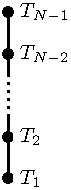
\includegraphics[scale=0.8]{chain3.pdf}
\end{minipage}
\begin{minipage}[c]{0.5\textwidth}
\centering
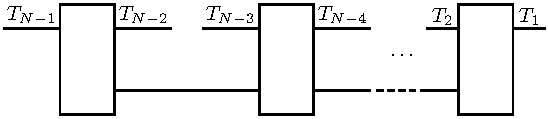
\includegraphics[scale=0.9]{general_comb_T.t1.pdf}
\end{minipage}
\end{center}

\medskip


The above diagram shows the chain and the corresponding comb in the case of quantum
objects. Note that the causal ordering of the spaces in the comb goes down the chain, so
the order is opposite.


\subsection{Connecting chains: the causal product}



It is easy to see that two chains can be appended to create a single chain using the
ordinal sum, and any chain
of more than one elements can be decomposed as an ordinal sum of  chains. Such operations are trickier for
chain types, since the chains have to be of even length. The next operation on boolean
functions will be suitable for such considerations. 
 
For a fixed decomposition $[n]=[n_1]\oplus[n_2]$ and functions
$f_1:\{0,1\}^{n_1}\to \{0,1\}$, $f_2:\{0,1\}^{n_2}\to \{0,1\}$, we define their {\em
causal product} as 
\[
f_1\vartriangleleft f_2:=f_1\otimes 1_{n_2}+p_{n_1}\otimes (f_2-1_{n_2}).
\]
For  $s^1\in \{0,1\}^{n_1}$ and $s^2\in \{0,1\}^{n_2}$, this function acts as
\begin{equation}\label{eq:causal_product}
(f_1\vtl f_2)(s^1s^2)= f_1(s^1)+p_{n_1}(s^1)(f_2(s^2)-1)=\begin{dcases} f_1(s^1), &
\text{ if } s^1\ne \theta_{n_1},\\
   f_2(s^2), & \text{ if } s^1=\theta_{n_1}.
   \end{dcases}
\end{equation}

%\begin{remark} Causal: can be interpreted as ''$f_1$ before $f_2$'' (actually after).
%
%
%\end{remark}
%
The following properties are immediate from \eqref{eq:causal_product}. 

\begin{lemma}\label{lemma:causal_product}
Let $f_1,g_1\in \Fe_{n_1}$, $f_2,g_2\in \Fe_{n_2}$. Then $f_1\vartriangleleft f_2\in \Fe_{n_1+n_2}$ and we
have 
\begin{enumerate}
\item[(i)] $(f_1\vtl f_2)^*=f_1^*\vtl f_2^*$,
\item[(ii)]$(f_1\vee g_1)\vtl (f_2\vee g_2)=(f_1\vtl f_2)\vee ( g_1\vtl g_2)=(f_1\vtl
g_2)\vee (g_1\vtl f_2)$,
\item[(iii)] $(f_1\wedge g_1)\vtl (f_2\wedge g_2)=(f_1\vtl f_2)\wedge ( g_1\vtl g_2)=(f_1\vtl
g_2)\wedge (g_1\vtl f_2)$.
\end{enumerate}
Moreover, for any $f_3\in \Fe_{n_3}$, and for the decomposition $[n]=[n_1]\oplus
[n_2]\oplus [n_3]$, we have 
\[
(f_1\vtl f_2)\vtl f_3=f_1\vtl (f_2\vtl f_3).
\]
\end{lemma}



We can also combine $f_1$ and $f_2$ in the opposite order:
\[
f_2\vtl f_1: =1_{n_1}\otimes f_2+(f_1-1_n)\otimes p_{n_2},
\]
so that
\begin{equation}\label{eq:causal_product_op}
(f_2\vtl f_1)(s^1s^2)=f_2(s^2)+p_{n_2}(s^2)(f_1(s^1)-1_{n_1})=\begin{dcases} f_2(s^2), & \text{ if }
s^2\ne \theta_{n_2},\\
   f_1(s^1), & \text{ if } s^2=\theta_{n_2}.
   \end{dcases}
\end{equation}
Of course, this product has similar properties as listed in the above lemma.
To avoid any confusion, we have to bear in mind the fixed decomposition $[n]=[n_1]\oplus
[n_2]$ and that for the concatenation $s=s^1s^2$, $f_i$ acts on $s^i$. 

\begin{lemma}\label{lemma:causal_tensor} In the situation as above, we have
\[
f_1\otimes f_2 = (f_1\vtr f_2)\wedge (f_2\vtr f_1).
\]

\end{lemma}


\begin{proof} This is again by straightforward computation from \eqref{eq:causal_product}
and \eqref{eq:causal_product_op}: let
$s^1\in \{0,1\}^{n_1}$, $s^2\in \{0,1\}^{n_2}$ and compute
\begin{align*}
(f_1\vtl f_2)\wedge (f_2\vtl
f_1)(s^1s^2)&=\left(f_1(s^1)+p_{n_1}(s^1)(f_2(s^2)-1)\right)\left(f_2(s^2)+p_{n_2}(s^2)(f_1(s^1)-1)\right)\\
=f_1(s^1)f_2(s^2),
\end{align*}
the last equality follows from the fact that $f_i(s^i)(1-f_i(s^i))=0$ (since $f_i(s^i)\in
\{0,1\}$) and the fact that $p_{n_1}$ is the least element in $\Fe_{n_1}$, so that
$p_{n_1}(s^1)(f_1(s^1)-1)=p_{n_1}(s^1)-p_{n_1}(s^1)=0$. 

\end{proof}

For the smallest and the largest element in $\Fe_n$, the causal product behaves as
follows.
\begin{lemma}\label{lemma:onechain_causal}
Let  $f\in \Fe_{n_1}$ and let $n_2\in \mathbb N$. Then for the decomposition
$[n_1+n_2]=[n_1]\oplus [n_2]$,  
\[
f\vtl 1_{n_2}= f\otimes 1_{n_2}\le 1_{n_2}\vtl f
\]
and
\[
p_{n_2} \vtl f= f \otimes p_{n_2}\le f\vtl p_{n_2}.
\]
In particular,
\[
(p_{n_1}\otimes 1_{n_2})^*=1_{n_1}\vtl p_{n_2}=1-p_{[n_1]}+p_{n_1+n_2}
\]
is the chain type for $\{\emptyset\subsetneq [n_1]\subsetneq [n_1+n_2]\}$. Similar
properties hold for the decomposition $[n_1+n_2]=[n_2]\oplus[n_1]$.
\end{lemma}

\begin{proof}
Immediate from the definition of the causal product and Lemma \ref{lemma:causal_tensor}.

\end{proof}







Using the last part of Lemma \ref{lemma:causal_product},
for a decomposition $[n]=\oplus_i[n_i]$ and $f_i\in \Fe_{n_i}$,  we may define the function $f_1\vtl\dots \vtl f_k\in
\Fe_{n}$. Note that we have for $s=s^1\dots s^k$, 
\begin{align*}
(f_1\vtl \dots\vtl f_k)(s)&=f_1(s^1)+p_{n_1}(s^1)(f_2(s^2)-1)+\dots + p_{n_1}(s^1)\dots
p_{n_{k-1}}(s^{k-1})(f_k(s^k)-1)\\
&= \begin{dcases} f_1(s_1) & \text{ if } s^1\ne \theta_{n_1}\\
f_2(s^2) & \text{ if } s^1=\theta_{n_1}, s^2\ne \theta_{n_2}\\
\dots & \\
f_k(s^k) & \text{ if } s^1=\theta_{n_1},\dots,  s^{k-1}=\theta_{n_{k-1}}.
\end{dcases}
\end{align*}
For any permutation $\pi\in \permut_k$, we define  $f_{\pi^{-1}(1)}\vtl \dots \vtl
f_{\pi^{-1}(k)}\in \Fe_n$ in an obvious way.


We will show that the causal product is related to the ordinal sum $\star$ of the corresponding
posets.

\begin{prop}\label{prop:vtl_ordinal} Let $f\in \Te_{n}$, $g\in \Te_{m}$
and
consider the decomposition $[n+m]=[n]\oplus[m]$. Replace the labels of $\Pe_g$ by their
translations $L_S\mapsto n+L_S=\{n+i,\ i\in L_S\}$.
Then  
\begin{enumerate}
\item[(a)] If $[n]\in \Pe_f$ and $\emptyset \in \Pe_g$, then $\Pe_{f\vtl g}=\Pe_f\star
(\Pe_g\setminus\{\emptyset\})$, with all labels remaining the same.
\item[(b)] If $[n]\in \Pe_f$ and $\emptyset \notin \Pe_g$, then $\Pe_{f\vtl
g}=(\Pe\setminus \{[n]\})\star \Pe_g$, where the labels of $[n]$ are added to the
labels of elements in $\mathrm{Min}(\Pe_g)$.
\item[(c)] If $[n]\notin \Pe_f$ and $\emptyset \in \Pe_g$, then $\Pe_{f\vtl g}=\Pe_f\star
(\Pe_g\setminus\{\emptyset\})$, where the free outputs  of $f$ are added to the label sets
of elements in $\mathrm{Min}(\Pe_g\setminus \emptyset)$.
\item[(d)] If $[n]\notin \Pe_f$ and $\emptyset \notin \Pe_g$, then $\Pe_{f\vtl
g}=\Pe_f\star \{\bullet\}\star \Pe_g$, where $\{\bullet\}$ is a one-element poset with
label $L_\bullet=O_f^F$.

\end{enumerate}

\end{prop}



\begin{proof} By definition of the causal product, we have  
\[
f\vtl g=\sum_{S\in \Pe_f\setminus\{[n]\}} \hat f_Sp_S+ (\hat f_{[n]}-1 + \hat
g_\emptyset)p_{[n]}+\sum_{T\in \Pe_g\setminus \{\emptyset\}} \hat g_T p_{[n]\oplus T}.
\]
The term in brackets can be equal to 1, -1, or 0, depending on whether $[n]\in \Pe_f$ and
$\emptyset\in \Pe_g$. The statement is now immediate.


\end{proof}

\begin{exm}
The following Hasse diagrams show some examples of the causal products in cases (a)-(d).
By  Proposition
\ref{prop:append_chain_f} below, all the results are type functions. 

\begin{center}
\begin{minipage}[c]{0.2\textwidth}
\centering
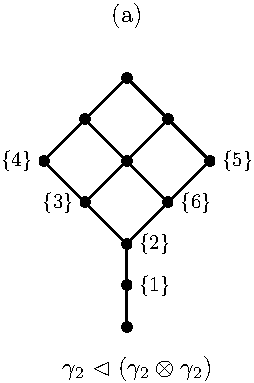
\includegraphics[scale=0.7]{vtl_a.pdf}
\end{minipage}
\begin{minipage}[c]{0.2\textwidth}
\centering
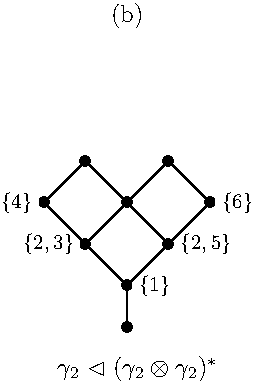
\includegraphics[scale=0.7]{vtl_b.pdf}
\end{minipage}
\begin{minipage}[c]{0.2\textwidth}
\centering
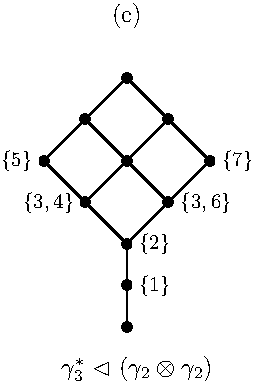
\includegraphics[scale=0.7]{vtl_c.pdf}
\end{minipage}
\begin{minipage}[c]{0.2\textwidth}
\centering
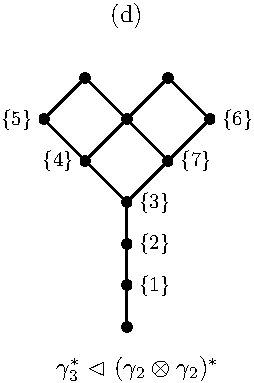
\includegraphics[scale=0.7]{vtl_d.pdf}
\end{minipage}
\end{center}



\end{exm}





It is not clear that if $f$ and $g$ are type functions, then $f\vtl g$ is a type function as well. 
Nevertheless, it can be seen from the above result
that if both $f$ and $g$ are chain types with chains of $N$ and $M$ elements,
respectively, then $f\vtl g$ is a chain type for a chain with $M+N\pm 1$
elements. Note also that that this construction can be
interpreted as appending the two chains in the respective order. 
Our next result shows that if $f$ or $g$ is a chain type, we always obtain a type
function.




\begin{prop}\label{prop:append_chain_f}  Let $f\in \Te_{n_1}$ and let $\beta\in \Te_{n_2}$
be a chain type. Then both $f\vtl \beta$ and $\beta\vtl f$ are types, with outputs
$O=O_f\oplus O_\beta$ and inputs $I=I_f\oplus I_\beta$. 

\end{prop}

\begin{proof} Let  $\beta=\sum_{k=1}^{N}(-1)^{k-1}p_{S_k}$
for some odd $N$ and $S_1\subsetneq \dots \subsetneq S_N\subseteq [n_2]$. We will proceed
by induction on $N$. Suppose $N=1$. If $S_1=\emptyset$,
then $\beta=1_{n_2}$ and we have by Lemma \ref{lemma:onechain_causal}
\[
f\vtl 1_{n_2}=f\otimes 1_{n_2}\in \Te_{n_1+n_2}
\]
and
\[
1_{n_2}\vtl f=(p_{n_2}\vtl f^*)^*=(f\otimes p_{n_2})^*\in \Te_{n_1+n_2}.
\]
Assume that  $S_1=[n_2]$, then $\beta=p_{n_2}$ and the assertion follows by duality. 
If $\emptyset\ne S_1\subsetneq [n_2]$, then we have $\beta\approx p_{m_1}\otimes
1_{m_2}=p_{m_1}\vtl 1_{m_2}$ for $m_1=|S_1|$, $m_1+m_2=n_2$. Then 
\[
\beta\vtl f\approx p_{m_1}\vtl (1_{m_2}\vtl f)\in \Te_{n_1+n_2},\quad f\vtl \beta\approx (f\vtl p_{m_1})\vtl 1_{m_2} \in
\Te_{n_1+n_2},
\]
by the first part of the proof and Lemma \ref{lemma:causal_product}.

Assume next that the assertion holds for all odd numbers $M<N$. Using Proposition
\ref{prop:vtl_ordinal} (d), we see that $\beta\approx \beta_1\vtl\beta_2$, where $\beta_1$ is
an $N-2$-element chain type and $\beta_2$ is a one-element chain  type. Then
\[
\beta\vtl f\approx \beta_1\vtl(\beta_2\vtl f),\qquad f\vtl\beta\approx (f\vtl\beta_1)\vtl\beta_2
\]
are type functions, by the induction assumption. 


To prove the statement on the output and input indices, note that for any $i\in [n_1]\oplus [n_2]$, we have  $e^i_{n_1+n_2}=e^j_{n_1}\theta_{n_2}$ or
$e^i_{n_1+n_2}=\theta_{n_1}e^k_{n_2}$
for some $j\in [n_1]$, $k\in [n_2]$. Then   
\[
f\vtl\beta(e^i)=f(e^j_{n_1})\ \text{ or } f\vtl \beta(e^i)=\beta(e^k_{n_2}).
\]
The statement on input/output indices  follow from Lemma \ref{lemma:fh_setting}. The proof
for $\beta\vtl f$ is similar. 

\end{proof}


\subsection{The structure of type functions}

Our main result here is the  following structure theorem for the type functions.


\begin{theorem}\label{thm:structure}
Let  $f\in \Te_n$. Then there is  a decomposition
$[n]=\oplus_{i=1}^k[n_i]$, chain types 
$\beta_1\in \Te_{n_1}$,\dots, $\beta_k\in
\Te_{n_k}$ such that $O_f=\oplus_j O_{\beta_j}$, $I_f=\oplus_j I_{\beta_j}$, finite index sets $A$, $B$ and permutations $\pi_{a,b}\in
\permut_k$, $a\in A$, $b\in B$ such that 
\[
f\approx \bigvee_{a\in A}\bigwedge_{b\in B} (\beta_{\pi^{-1}_{a,b}(1)}\vtl \dots \vtl
\beta_{\pi^{-1}_{a,b}(k)})=\bigwedge_{b\in B}\bigvee_{a\in A}(\beta_{\pi^{-1}_{a,b}(1)}\vtl \dots \vtl
\beta_{\pi^{-1}_{a,b}(k)}).
\]
%Moreover, there is a decomposition $[k]=\oplus_{j=1}^{l} [k_j]$, permutations $\sigma_c^j\in
%\permut_{k_j}$ and $\lambda_d\in \permut_l$ such that either $\pi_{c,d}$, $c\in A$, $d\in
%B$, or $\pi_{d,c}$, $d\in A$, $c\in B$
%are block permutation of the form
%\[
%\rho_{\lambda_d}\circ(\oplus_j\sigma_c^j)
%\]
%(see Appendix \ref{sec:permut}).
%
\end{theorem}


\begin{proof} We will once again proceed by induction on $n$. Since any element in $\Te_n$
for $n\le 3$ is a chain type, the statement clearly holds in this case. Assume the
condition holds for all $m<n$. The condition is obviously invariant under permutations. 
Assume $f$ can be written in the given form, then
\[
f^*\approx \bigwedge _{a\in A}\bigvee_{b\in B} (\beta^*_{\pi^{-1}_{a,b}(1)}\vtl \dots \vtl
\beta^*_{\pi^{-1}_{a,b}(k)})=\bigvee_{b\in B}\bigwedge_{a\in A} (\beta^*_{\pi^{-1}_{a,b}(1)}\vtl \dots \vtl
\beta^*_{\pi^{-1}_{a,b}(k)}).
\]
Since $\beta_j^*$ is a chain type for each $j$, this proves the statement for $f^*$. 

It is now enough to show this form for  $f=f_1\otimes f_2$, where 
$f_1\in \Te_m$, $f_2\in \Te_{n-m}$ with $[n]=[m]\oplus[n-m]$. By the induction assumption,
$f_1$ amd $f_2$ satisfy the conditions, so that
\begin{align*}
f_1&\approx\bigvee_{a\in A}\bigwedge_{b\in B} (\beta^1_{\pi^{-1}_{a,b}(1)}\vtl \dots \vtl
\beta^1_{\pi^{-1}_{a,b}(k_1)})=\bigwedge_{b\in B}\bigvee_{a\in A} (\beta^1_{\pi^{-1}_{a,b}(1)}\vtl \dots \vtl
\beta^1_{\pi^{-1}_{a,b}(k_1)}),\\
f_2&\approx\bigvee_{c\in C}\bigwedge_{d\in D} (\beta^2_{\tau^{-1}_{c,d}(1)}\vtl \dots \vtl
\beta^2_{\tau^{-1}_{c,d}(k_2)})=\bigwedge_{d\in D} \bigvee_{c\in C}(\beta^2_{\tau^{-1}_{c,d}(1)}\vtl \dots \vtl
\beta^2_{\tau^{-1}_{c,d}(k_2)})
\end{align*}
for some chain types  $\beta^1_j\in \Te_{m_j}$, $[m]=\oplus^{k_1}_{j=1}[m_j]$, and $\beta^2_j\in \Te_{l_j}$,
$[n-m]=\oplus_{j=1}^{k_2}[l_j]$ and permutations $\pi_{a,b}\in \permut_{k_1}$, $\tau_{c,d}\in
\permut_{k_2}$.
Let 
\[
\beta^{a,b}_1:=\beta^1_{\pi^{-1}_{a,b}(1)}\vtl \dots \vtl
\beta^1_{\pi^{-1}_{a,b}(k_1)},\qquad \beta^{c,d}_2:= \beta^2_{\tau^{-1}_{c,d}(1)}\vtl \dots \vtl
\beta^2_{\tau^{-1}_{c,d}(k_2)}.
\]
Using the   properties of the tensor product (Lemma \ref{lemma:fproduct})ii), we get from
Lemma \ref{lemma:causal_tensor}
\[
f\approx \bigl(\bigvee_{a\in A}\bigwedge_{b\in B}\beta_1^{a,b}\bigr)\otimes \bigl(\bigvee_{c\in
C}\bigwedge_{d\in D}\beta_2^{c,d}\bigr)=\bigvee_{a,c}\bigwedge_{b,d}
(\beta_1^{a,b}\otimes \beta_2^{c,d})=\bigvee_{a,c}\bigwedge_{b,d}(\beta_1^{a,b}\vtl
\beta_2^{c,d})\wedge (\beta_2^{c,d}\vtl \beta_1^{a,b})
\]
On the other hand, using Lemma \ref{lemma:causal_tensor} and Lemma
\ref{lemma:causal_product}, we
get
\begin{align*}
f&\approx \bigl(\bigwedge_{b\in B}\bigvee_{a\in A}\beta_1^{a,b}\bigr)\otimes \bigl(\bigwedge_{d\in D}\bigvee_{c\in
C}\beta_2^{c,d}\bigr)\\
&=\left[\bigl(\bigwedge_{b\in B}\bigvee_{a\in A}\beta_1^{a,b}\bigr)\vtl \bigl(\bigwedge_{d\in D}\bigvee_{c\in
C}\beta_2^{c,d}\bigr)\right]\wedge \left[\bigl(\bigwedge_{d\in D}\bigvee_{c\in
C}\beta_2^{c,d}\bigr)\vtl\bigl(\bigwedge_{b\in B}\bigvee_{a\in A}\beta_1^{a,b}\bigr)
\right]\\
&= \bigl(\bigwedge_{b,d}\bigvee_{a,c} \beta_1^{a,b}\vtl \beta_2^{c,d}\bigr) \wedge
\bigl(\bigwedge_{b,d}\bigvee_{a,c} \beta_2^{c,d}\vtl \beta_1^{a,b}\bigr).
\end{align*}
We have the decomposition $[n]=\oplus_{j=1}^k[n_j]$, with $k=k_1+k_2$ and $n_j=m_j$,
$j=1,\dots, k_1$,  $n_j=l_{j-k_1}$, $j=k_1+1,\dots,k$, and chain types $\beta_j\in
\Te_{n_j}$, $\beta_j=\beta_j^1$ for $j=1,\dots,k_1$ and $\beta_j=\beta^2_{j-k_1}$ for
$j=k_1+1,\dots,k$. To get the permutation sets, let $A'=A\times C$, $B'=B\times D\times
\permut_2$ and define $\pi_{a',b'}$ in $\permut_k$ as the block permutation with respect to the
decomposition $[k]=[k_1]\oplus[k_2]$ (see Appendix \ref{sec:permut})
\[
\pi_{(a,c),(b,d,\lambda)}=\rho_\lambda\circ(\pi_{a,b}\oplus \tau_{c,d}).
\]
This  finishes the proof.

\end{proof}


\begin{remark} In general, it is not clear for which sets of permutations such a
combination of chain types will be a chain type. Nevertheless, since all the connected
chains have the same input and output indices, a function of the form as in Theorem
\ref{thm:structure} will always be a subtype. That is, the objects corresponding to such a
function will describe a set of channels, obtained by taking pullback and pushouts of
combs.

\end{remark}

\subsection{The labelled poset $\Pe_f^0$}

Let $\Pe_f^0$ be the subposet in $\Pe_f$, consisting of the elements with nonempty labels
and $\emptyset$ if it is contained in $\Pe_f$. We will show that any $f\in \Te_n$ is fully determined by $\Pe_f^0$ (and
$n$). This is convenient, because $\Pe_f^0$ is much smaller and easier to visualise that $\Pe_f$. More
importantly, from $\Pe_f^0$, one can find a  decomposition of $f$ as products and complements
of other functions. In particular, it is possible to obtain from $\Pe_f^0$ some choice of
the chain types  $\beta_1,\dots,\beta_k$
in the decomposition in Theorem \ref{thm:structure}.


We will start by some basic properties of $\Pe_f^0$. Some further properties, and more
technical parts of the proofs, can be found in Appendix \ref{app:pf0}. 

Recall that for all $T\in \Pe_f$, we have $T=\cup\{L_{T'},\ T'\in \Pe_f^0, T'\subseteq
T\}$.


\begin{lemma}\label{lemma:p0_basic} Let $f\in \Te_n$.
\begin{enumerate}
\item[(i)] $\mathrm{Min}(\Pe_f^0)=\mathrm{Min}(\Pe_f)$.
\item[(ii)] $\Pe_f^0$ is a chain $\iff$  $\Pe_f$ is a chain $\iff$  $\Pe_f^0= \Pe_f$.

\item[(iii)] If $\Pe^0_f$ has a largest element,  then $f$ or $f^*$ has a free
output. In this case  the corresponding set is the largest element in $\Pe_f$. 

\end{enumerate}
\end{lemma}


\begin{proof} 
(i) Obvious. For (ii), assume that $\Pe^0_f$ is a chain and let $S,T\in \Pe_f$. Let $i\in
S\setminus T$ and $j\in T$, and let $S'\subseteq  S$ and $T'\subseteq  T$ be such that $S',T'\in
\Pe_f^0$ and $i\in L_{S'}$, 
$j\in L_{T'}$. Since $\Pe_f^0$ is a chain, $S'$ and $T'$ are comparable. If $S'\subseteq T'$,
then $S'\subseteq  T'\subseteq  T$, so that $i\in T$, which is not possible. Hence
$T'\subseteq S' \subseteq S$, for all $T'\in \Pe_f^0$, $T'\subseteq T$. Hence $T\subseteq
S$, and $\Pe_f$ is a chain. It is clear that then $\Pe_f^0=\Pe_f$.  

If $\Pe_f$ is not a chain, then there are some type
functions
$f_1$, $f_2$ such that $f=f_1\otimes f_2$ or $f=(f_1\otimes f_2)^*$. Moreover, the ranks
of $f_1$ and $f_2$ are at least 2. It follows that both $\Pe_{f_1\otimes f_2}$ and
$\Pe_{(f_1\otimes f_2)^*}$ contain an element $S\oplus T$, where $S\in \Pe_{f_1}$, $T\in
\Pe_{f_2}$ but none of the two elements is minimal. Then there is some $S'\in \Pe_{f_1}$
and $T'\in \Pe_{f_2}$ such that $S'\oplus T$, $S\oplus T'\subseteq S\oplus T$, so that no
element of $S\oplus T$ is a label. Hence
$S\oplus T\notin
\Pe_f^0$, so that $\Pe_f\ne \Pe_f^0$. 

To prove (iii) let $T$ be the largest element in $P^0_f$. Then 
\[
\cup\Pe_f=\cup L_S \subseteq T\subseteq \cup \Pe_f.
\]
 If follows that $T=\cup\Pe_f $ is the largest element in $\Pe_f$. If $T\ne [n]$, then
 clearly, $f$ has some free outputs. If $T=[n]$, then since $[n]\in \Pe_f^0$, we have
 $\emptyset\ne L_{[n],f}=O_{f^*}^F$, so that $f^*$ has free outputs.

\end{proof}



%We next describe the basic constructions on type functions in terms of $\Pe_f^0$.
%
%
%\begin{lemma}\label{lemma:p0_constr} Let $f\in \Te_{n}$, $g\in \Te_{m}$. 
%\begin{enumerate}
%\item[(i)] If $S\in \Pe_f^0$ and $S\ne \emptyset$, $S\ne [n]$, then $S\in \Pe^0_{f^*}$. 
% $\emptyset \in \Pe^0_f$ $\iff$ $\emptyset \notin \Pe^0_{f^*}$ and  $[n]\in
%\Pe^0_f$ $\iff$ $f^*$ has  free outputs.
%\item[(ii)] $\Pe^0_{f\otimes g}=\{S\oplus T:\ S\in \Pe_f^0,\ T\in \Pe_g^0, \ S\in
%\mathrm{Min}(\Pe_f) \text{ or } T\in \mathrm{Min}(\Pe_g)\}=: \Pe_f^0\oplus_{\min} \Pe_g^0$.
%
%\item[(iii)] The causal product $f\vtl g$ is connected with the ordinal sum $\star$ of
%posets as follows:
%\begin{enumerate}
%\item[(a)] If $\Pe_f^0$ has no largest element, then
%\[
%\Pe^0_{f\vtl g}=\Pe_f^0\star (\Pe_{g}^0\setminus \{\emptyset\})
%\]
%with same sets of labels.
%\item[(b)] If $[n]\in \Pe_f^0$, then 
%\[
%\Pe^0_{f\vtl g}=(\Pe_{f}^0\setminus \{[n]\})\star \Pe_g^0
%\]
%and for the minimal elements $S\in \mathrm{Min}(\Pe_g^0)$ the labels are
%replaced by $L_{S,g}\cup L_{[n],f}$.
%\item[(c)] If $\Pe_f^0$ has a largest element other than $[n]$ and $\emptyset \in \Pe_g$,
%then 
%\[
%\Pe^0_{f\vtl g}=\Pe_f^0\star(\Pe_{g}^0\setminus \{\emptyset\})
%\]
%and the free outputs of $f$ are added to the labels of elements in
%$\mathrm{Min}(\Pe_g^0\setminus\{\emptyset\})$.
%\item[(d)] If $\Pe_f^0$ has a largest element other than $[n]$ and $\emptyset \notin 
%\Pe_g$, then 
%\[
%\Pe^0_{f\vtl g} =\Pe_f^0\star \{[n]\}\star\Pe_g^0
%\]
%where the label set $L_{[n]}$ consists of free outputs of $f$, all other labels remain the
%same.
%
%\end{enumerate}
%
%
%
%\end{enumerate}
%
%
%\end{lemma}
%
%
%\begin{proof} (i) First two assertions are clear, the last equivalence was proved in the
%proof of Lemma \ref{lemma:p0_basic}(iii).
%The statement (ii) follows from the proof of Proposition \ref{prop:pfinput}. 
%
%For (iii) we use Proposition \ref{prop:vtl_ordinal}.
%Under the assumption in (a), $[n]\notin \Pe_f^0$ and $f$ has no free outputs, so that even
%if $[n]\in \Pe_{f\vtl g}$, it certaily has an empty label set, so that $[n]\notin
%\Pe_{f\vtl g}^0$. Under the assumption in [(b)], $\Pe_{f\le g}$ contains $[n]$ only if
%$\emptyset\in \Pe_g$, in any case, the labels of $[n]$ have to be added to the minimal
%elements in $\Pe_g^0$. Under the assumption in (c), $[n]\notin \Pe_{f\vtl g}$, but $f$ has some
%free outputs that appear for the first time in $[n]\oplus S$, $S\in
%\mathrm{Min}(\Pe_g^0\setminus \{\emptyset\})$. Finally, under the assumptions in (d)
%$[n]\in \Pe_{f\vtl g}$ is labelled by the free outputs of $f$.
%
%\end{proof}



\begin{prop}\label{prop:pf0_largest} Assume that $f\in \Te_n$ is such that $f$ or $f^*$
has a free output.   Then
either $f$ is a chain type, or there is some $h\in \Te_m$ such that both a$h$ and $h^*$
have no free outputs, and  a chain type $\beta\in \Te_{n-m}$ such that $f\approx h\vtl \beta$.

\end{prop}



\begin{proof} Assume that $\Pe_f^0$ has no largest element, then $[n]\notin \Pe_f^0$ and by Lemma
\ref{lemma:p0_basic}(iii) and its proof,  $f^*$ has no free outputs, so that we must have $O_f^F\ne \emptyset$. But
then $f\approx h\otimes 1_k=h\vtl 1_k$ with $k=|O_f^F|$, where $h\in \Te_{n-k}$ has no
free outputs. Since $\Pe_h^0\simeq \Pe_f^0$, $\Pe_h^0$ has no largest element, so that
$h^*$ has no free outputs as well. 

Assume that $\Pe_f^0$ has a largest element $T$. If $T=[n]$, then $f^*$ has some free outputs. Hence
$f^*\approx h_1\otimes 1_{k_1}$ for some $h_1\in \Te_{n-k_1}$ with no free outputs. It follows that
$f\approx (h_1\otimes 1_{k_1})^*=(h_1\vtl 1_{k_1})^*=h_1^*\vtl p_{k_1}$. 

If $T\ne [n]$, then, since $T$  
is also the largest element in $\Pe_f$, we see that $f$ has free outputs, so that
$f\approx h_1\otimes 1_{k_1}=h_1\vtl 1_{\k_1}$, where $h_1\in \Te_{n-k_1}$ is a type function with no
free outputs. Since $\Pe_{h_1}^0=\Pe_f^0$,  $T$ is the largest
element in $\Pe^0_{h_1}$, but this time $T=[n-k_1]$, so that we may use the first part of the
proof. We obtain that there is some $k_2$ and a type function  $h_2\in\Te_{n-k_1-k_2}$
with no free outputs such that 
\[
f\approx h_1\vtl 1_{k_1}=h_2^*\vtl p_{k_2}\vtl 1_{k_1}
\]
So far, we have written $f$ in the form $f=h\vtl \beta$, where $\beta$ is a chain type and
$h\in \Te_{n-k}$ for $k>0$ is such that $h^*$ has no free outputs. If $h$ has free
outputs, we  may proceed as above, replacing $f$ by $h$. Since $n$ is decreasing at each step, we
 either get to $n-k \le 3$, in which case $h$ must be a chain and therefore also $f=h\vtl
 \beta$ is a chain, or $\Pe^0_h$ has no largest element, in which case we finish  by the
 first paragraph of the proof.


\end{proof}

In the situation of the above Proposition, if $f$ is not a chain, $\Pe_h^0$ and  $\beta$ can be
seen from $\Pe_f^0$ as follows. 
Since $h$ has no free outputs and does not contain
$[m]$, we obtain from Proposition \ref{prop:vtl_ordinal} that $\Pe_f^0\approx \Pe_h^0\star
(\Pe_\beta\setminus\{\emptyset\})$, with the same sets of labels.
It follows that there exists a largest element in $\Pe_f^0$ with the property that
it covers more than one element. Let this element be $S$ and let $T_1,\dots, T_k$ be the
elements covered by $S$. There is a chain $S=S_1\lneq \dots \lneq S_K$, where $S_K$ is
the largest element in $\Pe_f^0$. We then have $\Pe_h^0\simeq \cup_j T_j^{\downarrow}$. 
If $K$ is even, add an element $S_0$ with empty
label at the bottom of the chain to obtain a chain of even length. This then corresponds
to the chain type.  Some examples are given below.


\begin{center}
\begin{minipage}[c]{0.3\textwidth}
\centering
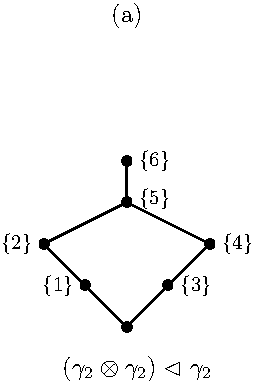
\includegraphics[scale=0.7]{fri_aa.pdf}
\end{minipage}
\begin{minipage}[c]{0.3\textwidth}
\centering
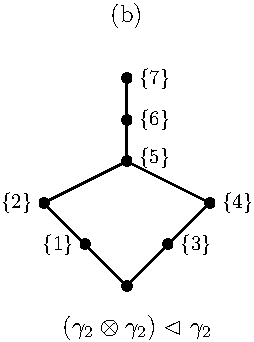
\includegraphics[scale=0.7]{fri_b.pdf}
\end{minipage}
\begin{minipage}[c]{0.3\textwidth}
\centering
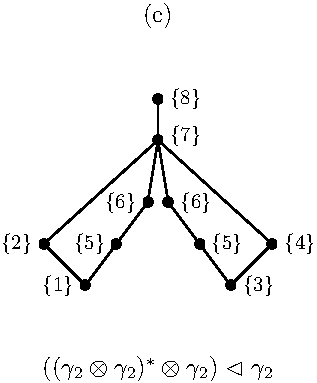
\includegraphics[scale=0.7]{fri_ccc.pdf}
\end{minipage}
\end{center}



\begin{prop}\label{prop:pf0_smallest} Let $f\in \Te_n$ be such that $f$ or
$f^*$ has a free input. 
Then either $f$ is a chain type, or there is some chain type $\beta\in
\Te_k$ and some $h\in \Te_{n-k}$ such that $h$ and $h^*$ have no free inputs and
$f\approx \beta\vtl
h$. 

\end{prop}


\begin{proof} Assume $f$ has a free input, $f\approx p_k\otimes
h=p_k\vtl h$,
where  $h\in \Pe_{n-k}$ has no free inputs. On the other hand, if $f^*$ has a
free input, then, similarly, $f^*\approx p_k\vtl g$ for some $g\in \Te_{n-k}$ with no free
inputs, hence $f\approx (p_k\vtl g)^*=1_k\vtl g^*$. Repeating the process, we get the result
after finitely many steps.


\end{proof}

Under the assumptions of the proposition above, assume that $f$ is not a chain type. 
Suppose that $\Pe_f^0$ has a least element $S_1$ and let $S$ be the smallest elemet in
$\Pe_f^0$ with the property that it is covered by more than one element. Let these
elements be $T_1,\dots, T_l$ and let  $S_1\lneq \dots \lneq S_K$ be a chain such that $S_K=S$.
Put $L:=\cap_j L_{T_j}$. 
Using
Proposition \ref{prop:vtl_ordinal} as before, we have the following situations. If  $L=\emptyset$, then put  $k=|S_K|$. 
If $K$ is odd, then the chain corresponds to a chain type
$\beta\in \Te_{k}$ and $\Pe_g^0=\cup_j T_j^{\uparrow}\cup\{\emptyset\}$. If $K$ is even, then $\Pe_g^0=\cup_j T_j^{\uparrow}$ and $\beta$
is the chain type for the chain $S_1\subsetneq \dots\subsetneq S_{K-1}$ (with free outputs
in $L_{S_K}$). If $L\ne \emptyset$, then add an element $S_{K+1}$ at the end of the chain, with label
$L_{S_{K+1}}=L$ and put $k=|S_{K+1}|$. If $K$ is odd, then $\beta\in \Te_k$ is the chain type for the chain
$S_1\lneq \dots \lneq S_K$ (with free outputs in $L$) and $\Pe_g^0=\cup_j
T_j^{\uparrow}\cup \{\emptyset\}$, with labels of $T_j$ replaced by $L_{T_j}\setminus L$.  If
$K$ is even, then $\Pe_g^0=\cup_j T_j^{\uparrow}$ and $\beta$ is the chain type  for
$S_1\subsetneq\dots\subsetneq S_{K+1}$.

If $\Pe_f^0$ has no least element, then by the assumptions $f$ must have free inputs (since $\Pe_{f^*}^0$
has least element $\emptyset$). Hence  $f\approx p_k\vtl g$, for $g\in \Te_{n-k}$ with no
free inputs. Note also that we have  $\emptyset
\notin \Pe_g$, so that $g^*$ has no free inputs as well. See the diagrams in Example \ref{exm:causal} (and the corresponding
subposets $\Pe_f^0$ of labelled elements) for some examples.




We will now deal with the case when $f$ and $f^*$ have no free indices.
Let $\Pe$ be a poset with labels in $[n]$ and let $\Pe_1,\Pe_2\subseteq \Pe$ be nonempty. We will say that $\Pe_1$ and $\Pe_2$ are {\em independent
components} of $\Pe$ if $\Pe=\Pe_1+\Pe_2$ (direct sum of posets) and $L_S\cap L_T=\emptyset$ for 
any $S\in \Pe_1$ and $T\in \Pe_2$. In this case, we will write
\[
\Pe=\Pe_1\indep \Pe_2.
\]


\begin{prop}\label{prop:nofree_components} Let $f\in \Te_n$ be such that $f$ and  $f^*$ have no
free indices. Assume that $\emptyset \notin \Pe_{f}$. 
\begin{enumerate}
\item[(i)] If $f^*\approx f_1\otimes f_2$ for some type functions $f_1$ and
$f_2$, then 
\[
\Pe_f^0\simeq (\Pe_{f_1}^0\setminus \emptyset) \indep  (\Pe_{f_2}^0\setminus
\emptyset).
\]
\item[(ii)] If $\Pe_f^0=\Pe_1\indep \Pe_2$ for some labelled subposets $\Pe_1$ and $\Pe_2$, 
then there are some type functions $f_1$ and $f_2$ such that $\Pe_1=(\Pe_{f_1}^0\setminus
\emptyset)$, $\Pe_2=(\Pe_{f_2}^0\setminus \emptyset)$ and
$f^*\approx f_1\otimes f_2$.
\item[(iii)] If $f\approx f_1\otimes f_2$ for type functions $f_1$ and
$f_2$, then no 
decomposition of $\Pe_f^0$ into independent components exists.

\end{enumerate}

\end{prop}

\begin{proof} Under the assumptions, $\Pe_{f^*}$ contains $\emptyset$ and has no largest
element.  Therefore
$\Pe_f^0=\Pe_{f^*}^0\setminus \{\emptyset\}$ and $\Pe_f^0$ has no largest or least
element.
Assume that $f_1\in \Te_{n_1}$ and $f_2\in \Te_{n_2}$ are such that $f^*=f_1\otimes f_2$
for the decomposition $[n]=[n_1]\oplus [n_2]$. Since $\emptyset \in
\Pe_{f^*}=\Pe_{f_1\otimes f_2}$, we see by Corollary \ref{coro:Pf} (iii) that both $\Pe_{f_1}$ and $\Pe_{f_2}$ must
contain $\emptyset$ and  $\Pe_{f^*}^0$ consists
of $\Pe_{f_1}^0$ and $\Pe_{f_2}^0$ glued at $\emptyset$, with labels of $\Pe_{f_2}^0$
translated by $n_1$. Since $\Pe_f^0=\Pe^0_{f^*}\setminus \{\emptyset\}$, the assertion (i) 
follows.  

For (iii), assume that $f=f_1\otimes f_2$ and $\Pe_f^0=\Pe_1\indep \Pe_2$. Note that none of
the functions can be a 1-element chain, since then $f$ would have free inputs or outputs. Let
$\mathrm{Min}(\Pe_{f_1})=\{U_1,\dots,U_k\}$,  $\mathrm{Min}(\Pe_{f_2})=\{V_1,\dots,V_l\}$.
By Corollary \ref{coro:Pf}(iii), we have  $\mathrm{Min}(\Pe_{f})=\mathrm{Min}(\Pe_{f_1})\times \mathrm{Min}(\Pe_{f_2})$. 
For some $i$ and $j$, let $(U_i,V_j)\in \Pe_1$. Since $(U_i,V_j)$ and $(T,V_j)$ are
comparable for any $T\in \Pe^0_{f_1}$, $U_i\le T$, we must have $(T,V_j)\in \Pe_1$ for all
such $T$. By Lemma \ref{lemma:pf0_mincover}, there is some $T$ that covers $U_i$. 
But then $L_{(T,V_j)}=L_{T,V_{j'}}=L_T$ for all $j'$, so that $(T,V_{j'})\in \Pe_1$
for all $j'$. Since $(U_i,V_{j'})\le (T,V_{j'})$ for all $j'$, this implies that $(U_i,
V_{j'})\in \Pe_1$ for all $j'$. By the same reasoning with $V_j$, we get that all $(U_i,
V_j)\in \Pe_1$, which is not posssible. 


For (ii), assume that $\Pe_f^0=\Pe_1\indep \Pe_2$. Since either $f$ or $f^*$ is, up to a
permutation, a tensor
product of type functions and we cannot have $f\approx f_1\otimes f_2$ by (iii), 
 it must hold that $f^*\approx f_1\otimes f_2$. But then by (i) $\Pe_f^0=\Pe'_1\indep \Pe'_2$, with 
$\Pe_i'=\Pe^0_{f_i}\setminus \{\emptyset\}$. Let 
\[
\Pe_f^0=\mathcal Q_1\indep \dots \indep  \mathcal Q_M
\]
be the finest decomposition into independent components. Then there are some $C,D\subset [M]$
such that 
\[
\Pe_1=\Indep_{i\in C} \mathcal Q_i,\quad  \Pe_2=\Indep_{i\in [M]\setminus C} \mathcal
Q_i, \quad \Pe'_1=\Indep_{i\in D} \mathcal Q_i,\quad  \Pe'_2=\Indep_{i\in [M]\setminus D}
\mathcal Q_i.
\]
Assume that $M\ge 3$, otherwise each $\Pe_i$ is one of $\Pe'_j$ and we are done. 
Then $D$ or $[M]\setminus D$ has at least two elements. So assume $|D|\ge 2$. Then $\Pe'_1$ has no largest
 element, which implies that $\Pe_1'=\Pe_{f_1}^0\setminus\{\emptyset\}=\Pe_{f_1^*}^0$ and $f_1^*$ satisfies the assumptions
 in (iii). Hence $f_1\approx g_1\otimes g_2$ for some type functions $g_1$ and $g_2$ and we
 obtain that 
 \[
\Pe_{g_1}^0\setminus \{\emptyset\} = +_{i\in D'}^L \mathcal Q_i,\quad \Pe_{g_2}^0\setminus
\{\emptyset\} = +_{i\in D\setminus D'}^L\mathcal Q_i
 \]
for some $D'\subset D$. Continuing in this way, we obtain that for any $i\in [M]$ there is
some type function $g_i$ such that $\emptyset \in \Pe_{g_i}^0$ and $\mathcal
Q_i=\Pe_{g_i}^0\setminus \{\emptyset\}$. It follows that 
\[
\Pe_1=+^L_{i\in C}(\Pe_{g_i}^0\setminus \{\emptyset\})=\Pe^0_{\otimes_{i\in
D}g_i}\setminus\{\emptyset\}
\]
and $f_1\approx \otimes_{i\in D}g_i$, similarly, $\Pe_2=\Pe^0_{\otimes_{i\in
[M]\setminus D}g_i}\setminus\{\emptyset\}$ and $f_2\approx\otimes_{i\in [M]\setminus
D}g_i$. 


\end{proof}

It follows that in the situation of the above Proposition, if $f^*\approx g_1\otimes
\dots\otimes g_k$, we can identify $\Pe_{g_l}^0$  by looking at the independent
components of $\Pe_f^0$.
\begin{exm}\label{exm:components} The next diagram shows $\Pe_f^0$ for a type function
$f\in \Te_{16}$:

\begin{center}
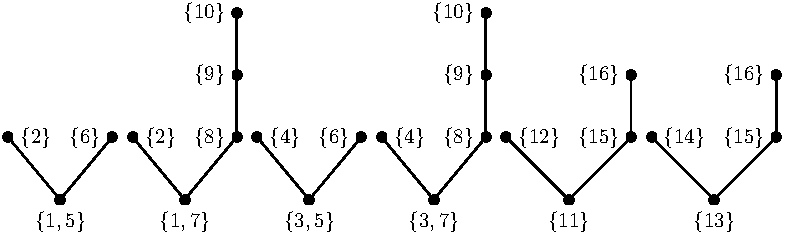
\includegraphics[scale=0.8]{components.pdf}
\end{center}

Note that $\Pe_f^0$ has no largest or smallest element, and also no free indices, so the
assumptions of Proposition \ref{prop:nofree_components} are satisfied. As a poset, $\Pe_f^0$  is a direct sum of 6 posets, but there are only two independent
components: one with labels $\le 10$, and one with labels  $>10$. It follows that
$f^*\approx
g_1\otimes g_2$. We can obtain
$\Pe_{g_1}^0$ and $\Pe_{g_2}^0$ by adding $\emptyset$, that is, an unlabelled minimal
element to each component, and relabelling if necessary:
\begin{center}
\begin{minipage}[c]{0.6\textwidth}
\centering
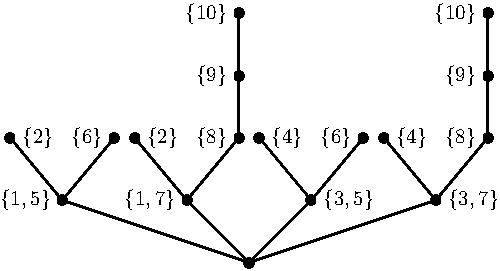
\includegraphics[scale=0.8]{component1.pdf}
\end{minipage}
\begin{minipage}[c]{0.35\textwidth}
\centering
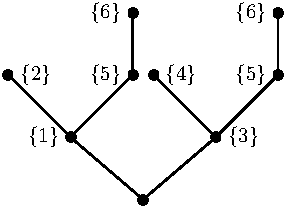
\includegraphics[scale=0.8]{component2.pdf}
\end{minipage}
\end{center}
We can also see that both $g_1^*$ and $g_2^*$ are products. Using the procedure described
in Appendix \ref{app:pf0}, we obtain that $g_1\approx ((\gamma_2\otimes \gamma_2)^*\otimes (\gamma_2\otimes
\gamma_4)^*)^*$ and $g_2\approx ((\gamma_2\otimes\gamma_2)^*\otimes \gamma_2)^*$.




\end{exm}


 The case when $\Pe_f^0$ has no independent components is somewhat more complicated.
 By the proposition  above, this
is the case when $f\approx f_1\otimes\dots\otimes f_k$. The proof of the following result is in Appendix \ref{app:pf0}.

\begin{prop}\label{prop:nofree_product}  Let $f\in \Te_n$ be such that $f$ and $f^*$ have
no free indices and $\emptyset\notin \Pe_f^0$. Assume $f\approx f_1\otimes
\dots\otimes f_k$ is a finest decomposition of $f$ as a product.  Then the labelled posets
$\Pe_{f_l}^0$, $l=1,\dots,k$ can be obtained from the structure of $\Pe_f^0$, up to a
permutation on the labels.

\end{prop}



\begin{theorem}\label{thm:pf0} Every type function $f\in \Te_n$ is fully determined by the
labelled poset $\Pe_f^0$.  

\end{theorem}

\begin{proof}  We will proceed by induction on
$n$. If $f$ is a chain type, the assertion follows from Lemma
\ref{lemma:p0_basic} and Proposition \ref{thm:graded}, so that the assertion holds for
$n\le 3$. Assume it is true for all $m<n$ and let $f\in \Te_n$. By Propositions
\ref{prop:pf0_largest} and \ref{prop:pf0_smallest} and remarks below them, if $f$ or
$f^*$ has
some free indices, then we have $f\approx \beta_1\vtl h \vtl \beta_2$, where $\beta_1,\beta_2$
are chain types and $h\in \Te_m$ is such that $h$ and $h^*$ do not have any free indices.
Moreover,  the chain types and $\Pe_h^0$ 
 can be obtained from $\Pe_f^0$. Since $m<n$,  $h$ is
 determined by $\Pe_h^0$ by the induction assumtions, so we are done.


If both $f$ and $f^*$ have no free indices, we may assume that $\emptyset \notin \Pe_f$, otherwise we 
replace $f$ by $f^*$. Then if $\Pe_f^0$ has independent components, we have
$f^*\approx f_1\otimes f_2$ for some type functions $f_i\in \Te_{n_i}$, $i=1,2$ and $n=n_1+n_2$,
such that the components have the form $\Pe_{f_i}^0\setminus \{\emptyset\}$. Since
$n_1,n_2<n$, we are done. If $\Pe_f^0$ has no independent components, then
$f\approx f_1\otimes\dots \otimes f_k$ for some $f_i\in \Te_{m_i}$, $i=1,\dots,k$, $m_1+\dots
+m_k=n$, and we obtin   $\Pe_{f_l}^0$ for all $l=1,\dots,k$ from $\Pe_f^0$ by Proposition
\ref{prop:nofree_product}. Again, the assertion follows by applying induction assumption
on each $f_l$.


\end{proof}

Using repeatedly the prodecure described in the above proof, we get to the situation when
all the obtained components are necessarily chains. In this way, we get a decomposition of $f$ into
chain types, together with a recipe how to construct $f$ from these chain types by using
tensor products, complements  and causal products. It is then clear, using also the proof
of Theorem \ref{thm:structure}, that these chain types give us a choice of
$\beta_1,\dots,\beta_k$ in the structure theorem \ref{thm:structure}.




\section{Conclusions}





\appendix


\section{Some basic definitions}
%Permutations, binary strings and boolean functions}


For $m\le n\in \mathbb N$, we will denote the corresponding interval $\{m,m+1,\dots,n\}$ by
$[m,n]$. For $m=1$, we will simplify to  $[n]:=[1,n]$. Let $\permut_n$ denote the set of all permutations of $[n]$.


\subsection{Block permutations}
\label{sec:permut}


 For $n_1,n_2\in \mathbb N$, $n_1+n_2=n$, 
we will denote by $[n]=[n_1]\oplus [n_2]$ the decomposition of $[n]$ as a concatenation of two 
intervals
\[
[n]=[n_1][n_1+1,n_1+n_2].
\]
Similarly, for $n=\sum_{j=1}^kn_j$, we have the decomposition
\[
[n]=\oplus_{j=1}^k[n_j]=[m_1,m_1+n_1][m_2,m_2+n_2]\dots[m_k,m_k+n_k],
\]
where $m_j:=\sum_{l=1}^{j-1} n_j$ (so $m_1=0$). Note that the order of $n_1,\dots, n_k$ in
this decomposition is
fixed. 

We have two kinds of special permutations related to the above decomposition. For
$\sigma_j\in \permut_{n_j}$, we denote by $\oplus_j \sigma_j\in \permut_n$ the permutation that acts as
\[
m_j+l\mapsto m_j+\sigma_j(l),\qquad l=1,\dots,n_j,\ j=1,\dots, k. 
\]
On the other hand, we have for any $\lambda\in \permut_k$ a unique permutation
$\rho_\lambda\in\permut_n$  such that $\rho_\lambda^{-1}$ acts as
\[
[m_1,m_1+n_1][m_2,m_2+n_2]...[m_k,m_k+n_k]\mapsto
[m_{\lambda(1)}+n_{\lambda(1)}][m_{\lambda(2)}+n_{\lambda(2)}]\dots[m_{\lambda(k)}+n_{\lambda(k)}]
\]
Note that we have
\[
\rho_\lambda\circ(\oplus_j\sigma_j)=(\oplus_j \sigma_{\lambda(j)})\circ\rho_\lambda.
\]
(These permutations  come from the operadic structure on the set of
all permutations $\permut_*$. See [Leinster, Higher operads] for the definition of and operad.)



\subsection{Partially ordered sets}\label{app:poset}

An overall reference for this section is [stanley].


A partially ordered set, or a {\em poset}, is a set $\Pe$ endowed with a reflexive, antisymmetric and
transitive relation $\le$, called the partial order. We will only encounter  the situation
when $\Pe$ is finite. A basic example of a poset is the set $\Pe(X)$ of all subsets of a
finite set $X$, ordered by inclusion. If $X=[n]$, we will denote $\Pe(X)$ by $2^n$. 

A subposet in a poset $\Pe$ is a $\mathcal Q\subseteq \Pe$ endowed with the partial order
relation inherited from $\Pe$. For any subset $\mathcal R\subseteq \Pe$, we define two
special 
subposets in $\Pe$ as
\[
\mathcal R^\downarrow=\{p\in \Pe,\ p\le r \text{ for some } r\in \mathcal R\}, \ \mathcal
R^\uparrow=\{p\in \Pe,\ p\ge  r \text{ for some } r\in \mathcal R\}.
\]

The set of minimal elements in $\Pe$ will be denoted by $\mathrm{Min}(\Pe)$. 
For elements $p,q\in \Pe$, we say that $q$ covers $p$, in notation $p\cover q$,  if $p\le q$
and for any $r$ such that $p\le r\le q$ we have $r=p$ or $r=q$. If $p$ covers a minimal
element, we will say that $p$ is a minimal covering element.


A totally ordered subposet $\Ce\subseteq \Pe$ is called a chain in $\Pe$. Such a chain  is
maximal if it is not contained in any other chain in $\Pe$.
The length of a chain $\Ce$ is defined as $|\Ce|-1$. 

We say that a poset $\Pe$  is graded of rank
$k$ if every maximal chain in $\Pe$ has the same length equal to $k$. Equivalently,  there is
a unique rank function $\rho: \Pe\to \{0,1,\dots,k\}$ such that $\rho(p)=0$ if $p$ is a
minimal element of $\Pe$ and $\rho(q)=\rho(p)+1$ if $p\cover q$. Basic examples of graded
posets are chains, antichains and $2^n$.


If $\Pe$ and $\mathcal Q$ are posets with disjoint sets, their direct sum $\Pe+\mathcal Q$ is a poset defined as 
the disjoint union $\Pe\cup \mathcal Q$, such that the order is preserved in each
component and elements in different components are incomparable. 
 Another way to compose
$\Pe$ and $\mathcal Q$ is the ordinal sum $\Pe\star \mathcal Q$, where the underlying set
is again the union $\Pe\cup \mathcal Q$ and the order in each component is preserved, but
for $p\in \Pe$ and $q\in \mathcal Q$ we have $p\le q$. A third way to compose posets that
we will use is the direct product $\Pe\times \mathcal Q$, where the underlying set is the
cartesian product $\Pe\times \mathcal Q$, with $(p_1,q_1)\le (p_2,q_2)$ if $p_1\le p_2$ in
$\Pe$  and $q_1\le q_2$ in $\mathcal Q$.
If $\Pe_1$ and $\Pe_2$ are graded posets with rank functions $\rho_1$ and $\rho_2$, then 
$\Pe_1\times \Pe_2$ is graded as well, with rank function $\rho$ given as
\[
\rho(p_1,p_2)=\rho_1(p_1)+\rho_2(p_2).
\]

The Hasse diagram of a finite poset $\Pe$ is a graph whose vertices are elements of $\Pe$
and there is an edge between $p$ and $q$ if $p\cover q$, and if $p\lneq r$, then $r$ is drawn above
$p$. Two posets are isomorphic if and only if they have the same Hasse diagrams. 


\subsection{Binary strings}

A binary string of length $n$ is a sequence  $s=s_1\dots s_n$, where $s_i\in
\{0,1\}$. Such a string can be interpreted as an element $\{0,1\}^n$, but also as a 
map $[n]\to \{0,1\}$, or a subset in  $[n]:=\{1,\dots,n\}$. It will be convenient to use
all these interpretations, but we will distinguish between them. The strings in
$\{0,1\}^n$ will be denoted by small letters, whereas the corresponding subsets of $[n]$
will be denoted by the corresponding capital letters. More specifically, for $s\in \{0,1\}^n$ and 
$T\subseteq [n]$, we denote
\begin{equation}\label{eq:string_subset}
S:=\{i\in [n],\ s_i=0\},\qquad t:=t_1\dots t_n,\ t_j=0 \iff j\in T.
\end{equation}
As usual, the set of all subsets of $[n]$ will be denoted by $2^n$. 
%We will also use the notation $2:=2^1=\{0,1\}$. 
With the inclusion ordering and complementation $S^c:=[n]\setminus S$,
$2^n$ is a boolean algebra, with the smallest element $\emptyset$ and largest element
$[n]$.  

The group $\permut_n$ has an obvious action on $\{0,1\}^n$. Indeed,
 for a string $s$  interpreted as a map $[n]\to 2$, we may define the action of
$\sigma\in \permut_n$ by precomposition as
\[
\sigma(s):=s\circ\sigma^{-1}=s_{\sigma^{-1}(1)}\dots s_{\sigma^{-1}(n)}.
\]
Note that in this way we have $\rho(\sigma(s))=(\rho\circ \sigma)(s)$. For a decomposition
$[n]=\oplus_{j=1}^k[n_j]$, we have a corresponding decomposition of
any string $s\in \{0,1\}^n$ as a concatenation of strings
\[
s=s^1\dots s^k,\qquad s^j\in \{0,1\}^{n_j}.
\]
For permutations $\sigma_j\in \permut_{n_j}$ and  $\lambda\in
\permut_k$, we have
\[
\rho_\lambda\circ(\oplus_j\sigma_j)(s^1\dots s^k)=\rho_\lambda(\sigma_1(s^1)\dots
\sigma_k(s^k))=\sigma_{\lambda(1)}(s^{\lambda(1)})\sigma_{\lambda(2)}(s^{\lambda(2)})\dots
\sigma_{\lambda(k)}(s^{\lambda(k)}).
\]





\subsection{Boolean functions and the  M\"obius transform}
\label{sec:boolean}

A function $f:\{0,1\}^n\to \{0,1\}$ is called a boolean function. 
The set of boolean functions, with pointwise ordering and complementation given by the
negation $\bar f=1-f$,  is a boolean algebra that can be identified with $2^{2^n}$.
We will denote the maximal element (the constant 1 function) by $1_n$. Similarly,
we denote the constant zero function by $0_n$.  For boolean
functions $f,g$, the pointwise minima and maxima will be denoted by $f\wedge g$ and $f\vee
g$. It is easily seen that we have
\begin{equation}\label{eq:wedgevee_fun}
f\vee g= f+g-fg,\qquad f\wedge g=fg,
\end{equation}
all the operations are pointwise. We now introduce and important example. 


\begin{exm}\label{ex:pS}
For $S\subseteq [n]$, we define
\[
p_S(t)=\Pi_{j\in S}(1-t_j),\qquad t\in \{0,1\}^n.
\]
That is, $p_S(t)=1$ if and only if $S\subseteq T$. In particular,
$p_\emptyset=1_n$ and $p_{[n]}$ is the characteristic function of the zero string.
Clearly, for $S,T\subseteq [n]$ we have $p_{S\cup T}=p_Sp_T=p_S\wedge p_T$, in particular,
$p_S=\Pi_jp_{\{j\}}$. 
\end{exm}

By the M\"obius transform, all boolean functions can be expressed as combinations of the functions $p_S$, $S\subseteq
[n]$ from the previous example.

\begin{theorem}\label{thm:mobius} Any $f:\{0,1\}^n\to 2$ can be expressed  in the form 
\[
f=\sum_{S\subseteq [n]} \hat f_Sp_S
\]
in a unique way. The coefficients  $\hat f_S\in \mathbb R$ obtained as
\[
\hat f_S=\sum_{\substack{t\in \{0,1\}^n\\ t_j=1, \forall  j\in S^c}} (-1)^{\sum_{j\in
S}t_j}f(t).
\]

\end{theorem}

\begin{proof}  By the M\"obius inversion formula (see [Stanley, Sec. 3.7] for details),
functions $f, g: 2^n\to \mathbb R$ satisfy
\[
f(S)=\sum_{T\subseteq S} g(T),\qquad S\in 2^n
\]
if and only if 
\[
g(S)=\sum_{T\subseteq S}(-1)^{|S\setminus T|} f(T).
\]
We now express this in terms of the corresponding strings $s$ and $t$.
It is easily seen that $T\subseteq S$ if and only if
$s_j=0$ for all $j\in T$, equivalently, $t_j=1$ for all $j\in S^c$. Moreover,
in this case we have  $|S\setminus T|=\sum_{j\in S} t_j$. This shows that $g(S)=\hat f_S$,
as defined in the statement. The first equality now gives
\[
f(s)=f(S)=\sum_{T\subseteq S} g(T)=\sum_{T:s_i=0,\forall i\in T}\hat f_T=\sum_{T:
p_T(s)=1}\hat f_T=\sum_{T\subseteq [n]} \hat f_Tp_T.
\]
For uniqueness, assume that $f=\sum_{T\subseteq [n]} c_Tp_T$ for some coefficients $c_T\in
\mathbb R$. Then 
\[
f(s)=\sum_{T: p_T(s)=1}c_T=\sum_{T\subseteq S}c_T.
\]
Uniqueness now follows by  uniqueness in the M\"obius inversion formula.

\end{proof}





%For a string $x\in \{0,1\}^n$ and any set of indices $\{i_1,\dots,i_k\}\subseteq [n]$, we
%will denote by $x^{i_1\dots i_k}$ the string in $\{0,1\}^{n-k}$ obtained from $x$ by removing
%$x_{i_1},\dots, x_{i_k}$. 

\subsection{The boolean algebra $\Fe_n$}


Let us introduce the subset of boolean functions 
\[
\Fe_n:=\{f:\{0,1\}^n\to 2,\ f(\theta_n)=1\},
\]
where we use $\theta_n$ to denote the zero string $00\dots 0$. 
In other words, $\Fe_n$ is the interval of all elements greater than $p_{[n]}$ in the boolean algebra 
$2^{2^n}$ of all boolean functions. With the pointwise ordering, $\Fe_n$ is a distributive lattice, with top element $1_n$ and 
 bottom element $p_n:=p_{[n]}$. We also define complementation  in $\Fe_n$ as
\[
f^*:=1_n-f+p_n.
\]
It can be easily checked that with these structures $\Fe_n$ is a boolean algebra, though
it is not a subalgebra of $2^{2^n}$.

Note that $p_S\in \Fe_n$ for any $S\subseteq [n]$, so in particular for $[k]$, with $k\le
n$. If $k<n$, we denote these functions as before by $p_{[k]}$, using the notation $p_n$
only for the distinguished top element.






We now introduce some more operations in $\Fe_n$. For $f\in \Fe_n$ and any permutation
$\sigma\in \permut_n$, we clearly have $f\circ \sigma\in \Fe_n$.
Further, let $f\in \Fe_{n_1}$ and $g\in \Fe_{n_2}$. With the decomposition
$[n_1+n_2]=[n_1]\oplus [n_2]$
and the corresponding concatenation of strings $s=s^1s^2$,  we define
the function $f\otimes g\in \Fe_{n_1+n_2}$ as
\[
(f\otimes g)(s^1s^2)=f(s^1)g(s^2),\qquad s^1\in \{0,1\}^{n_1},\ s^2\in \{0,1\}^{n_2}.
\]
Let $\lambda\in \permut_2$ be the transposition, then we have for any $f\in \Fe_{n_1}$ and
$g\in \Fe_{n_2}$
\[
(g\otimes f)=(f\otimes g)\circ \rho_\lambda,
\]
where $\rho_\lambda$ is the block permutation defined in  Section \ref{sec:permut}.

If $f,g\in \Fe_n$ are such that $g=f\circ\sigma$ for some $\sigma\in \permut_n$, we write
$f\approx g$. It is easily observed that if $f_1\approx g_1$ and $f_2\approx g_2$, then
$f_1\otimes f_2\approx g_1\otimes g_2$ and if $f\approx g$ then also $f^*\approx g^*$.


We now show some further important properties of these operations.

\begin{lemma}\label{lemma:fproduct} For $f\in \Fe_{n_1}$ and  $g,h\in \Fe_{n_2}$, we have
\begin{enumerate}
\item[(i)] $f\otimes g\le (f^*\otimes g^*)^*$, with equality if and only if either
$f=1_{n_1}$ and $g=1_{n_2}$, or $f=p_{n_1}$ and $g=p_{n_2}$.
\item[(ii)] $f\otimes (g\vee h)= (f\otimes g)\vee (f\otimes h)$, $f\otimes (g\wedge h)=
(f\otimes g)\wedge (f\otimes h)$.
\end{enumerate}

\end{lemma}

\begin{proof} The inequality in (i) is easily  checked, since $(f\otimes g)(s^1s^2)$ can be 1 only if
$f(s^1)=g(s^2)=1$. If both $s^1$ and $s^2$ are the zero strings, then $s^1s^2=\theta_{n_1+n_2}$ and both sides
are equal to 1. Otherwise, the condition $f(s^1)=g(s^2)=1$ implies that $(f^*\otimes
g^*)(s^1s^2)=0$, so that the right hand side must be 1. If $f$ and $g$ are both
constant 1, then 
\[
(1_{n_1}\otimes 1_{n_2})^*=1_{n_1+n_2}^*=p_{n_1+n_2}=p_{n_1}\otimes
p_{n_2}=1_{n_1}^*\otimes 1_{n_2}^*,
\]
in the case when both $f$
and $g$ are the minimal elements equality  follows by
duality. Finally, asume the equality holds and that $f\ne 1_{n_1}$, so that there is some $s^1$ such that 
$f(s^1)=0$. But then $s^1\ne \theta_{n_1}$, so that $f^*(s_1)=1$  and for any $s^2$,
\[
0=(f\otimes g)(s^1s^2)=(f^*\otimes
g^*)^*(s^1s^2)=1-f^*(s^1)g^*(s^2)+p_{n_1+n_2}(s^1s^2)=1-g^*(s^2),
\]
which implies that $g(s^2)=0$ for all $s^2\ne\theta_{n_2}$, that is, $g=p_{n_2}$. By the same argument,
$f=p_{n_1}$ if $g\ne 1_{n_2}$, which implies that either $f=1_{n_1}$ and $g=1_{n_2}$, or
$f=p_{n_1}$ and $g=p_{n_2}$.

The statement (ii) is easily proved from \eqref{eq:wedgevee_fun}.

\end{proof}

Consider the decomposition $[n]=[n_1]\oplus [n_2]$ and let $S\subseteq [n_1]$,
$T\subseteq [n_2]$. We then denote by $S\oplus T$ the disjoint union 
\begin{equation}\label{eq:disu}
S\oplus T:=S\cup (n_1+T)=S\cup\{n_1+j,\ j\in T\}.
\end{equation}
We summarize some easy properties of the basic functions $p_S$, $S\subseteq [n]$.

\begin{lemma}\label{lemma:PSPT}
\begin{enumerate}
\item[(i)] For $S,T\subseteq [n]$, we have $S\subseteq T$ $\iff$ $p_T\le p_S$ $\iff$
$p_Sp_T=p_S$.
\item[(ii)] For $S\subseteq [n]$, $\sigma\in \permut_n$,
$p_S\circ\sigma=p_{\sigma^{-1}(S)}$.
\item[(iii)] For $S\subseteq [n_1]$ and $T\subseteq [n_2]$, $p_S\otimes p_T=p_{S\oplus T}$.

\end{enumerate}
\end{lemma}

Let $f\in \Fe_n$ and let $\hat f$ be the M\"obius transform. Note that since $f$ has
values in $\{0,1\}$, we have by the proof of Theorem \ref{thm:mobius}
\[
\forall S\in 2^n, \quad \sum_{T\subseteq S} \hat f_T=f(s)\in \{0,1\}; \qquad \sum_{T\in 2^n} \hat
f_T=f(\theta_n)=1.
\]



\begin{prop}\label{prop:mobius} 

\begin{enumerate}
\item[(i)] For $f\in \Fe_n$ and  $\sigma\in \permut_n$, 
$\widehat{(f\circ \sigma)}_S=\hat f_{\sigma(S)}, \qquad S\subseteq [n]$.
\item[(ii)] For $f\in \Fe_n$, $\widehat{f^*}_S=\begin{dcases} 1-\hat f_S & S=\emptyset\text{ or } S=[n],\\
-\hat f_S & \text{otherwise}.
\end{dcases}$
\item[(iii)] For $f\in \Fe_{n_1}$, $g\in \Fe_{n_2}$, we have 
$\widehat{(f\otimes g)}_{S\oplus T}=\hat f_S\hat g_T$, $S\subseteq [n_1]$, $T\subseteq
[n_2]$.
%\item[(iv)] For $f,g\in \Fe_n$, we have
%\[
%\widehat{(f\wedge g)}_S=\sum_{T\subseteq S} \hat f_T\hat g_{S\setminus T}.
%\]
%\item[(v)] For $f,g\in \Fe_n$, we have
%\[
%\widehat{(f\vee g)}_S=\hat f_S+\hat g_S-\sum_{T\subseteq S} \hat f_T\hat g_{S\setminus T}.
%\]
%
\end{enumerate}


\end{prop}

\begin{proof} All statements follow easily from Lemma \ref{lemma:PSPT} and the uniqueness part in Theorem
\ref{thm:mobius}. 


\end{proof}

\section{Affine subspaces}
\label{sec:app_affine}
Let $V$ be a finite dimensional real vector space. A subset $A\subseteq V$ is an {\em affine
subspace} in $V$ if for any choice of  $a_1,\dots, a_k\in A$ and  $\alpha_1,\dots,\alpha_k\in \mathbb R$
such that $\sum_i\alpha_i=1$, we have $\sum_i\alpha_i a_i\in A$. It is clear that
$A=\emptyset$ is trivially an affine subspace.  Moreover, any linear subspace in $V$ is an affine subspace,
and an
affine subspace $A$ is linear if and only if $0\in A$. If $A \neq\emptyset$ and also
$0\notin A$, we say that $A$ is {\em proper}. 

A proper  affine subspace $A\subseteq V$ can be determined in two ways. Let 
\[
\lin(A):=\{a_1-a_2,\ a_1,a_2\in A\}.
\]
It is easily verified that $\lin(A)$ is a linear subspace, moreover, for any $a\in A$, we
have
\begin{equation}\label{eq:affine_l}
\lin(A)=\{a_1-a,\ a_1\in A\},\qquad A=a+\lin(A).
\end{equation}
We put $\dim(A):=\dim(\lin(A))$, the dimension of $A$. 

Let $V^*$ be the vector space dual of $V$ and let $\<\cdot,\cdot\>$ be the
duality. For a subset $C\subseteq V$, put
\[
C^*:=\{v^*\in V^*,\ \<v^*,a\>=1,\ \forall a\in A\}.
\]
Let $\tilde a\in A^*$ be any element and let $\Span(A)$ be the linear span of $A$ in
$V$. We then have
\begin{equation}\label{eq:affine_s}
A=\Span(A)\cap \{\tilde a\}^*,
\end{equation}
independently of $\tilde a$. The relation between the two expressions for $A$, given by
\eqref{eq:affine_l} and \eqref{eq:affine_s} is obtained as
\begin{equation}\label{eq:LandS}
\Span(A)=\lin(A)+\mathbb R\{a\},\qquad \lin(A)=\Span(A)\cap \{\tilde a\}^\perp,
\end{equation}
independently of $a\in A$ or $\tilde a\in A^*$. Here $+$ denotes the direct sum of
the vector spaces and $C^\perp$ denotes the annihilator of a set $C$.
The following lemma is  easily proven.

\begin{lemma}\label{lemma:dual} Let $C\subseteq V$ be any subset. Then $C^*$ is an affine subspace in 
$V^*$ and we have
\[
0\in C^* \iff C= \emptyset, \qquad C^*=\emptyset\iff 0\in \aff(C).
\]
Assume $C\ne \emptyset$ and $0\notin \aff(C)$. Then
\begin{enumerate}
\item[(i)] $C^*$ is proper and we have $\lin(C^*)=C^\perp=\Span(C)^\perp$,
\item[(ii)] $\aff(C)=C^{**}$ and for any $c_0\in
C$, we have
\begin{align*}
\lin(C):= \Span\{c_1-c_2,\ c_1,c_2\in C\}=\Span\{c-c_0,\ c\in C\}=\lin(C^{**}).
\end{align*}

\end{enumerate}


\end{lemma}

\begin{coro}\label{coro:dual} Let $A\subseteq V$ be a proper affine subspace. Then 
\begin{enumerate}
\item[(i)] $A^*$ is a proper affine subspace in $V^*$ and $A^{**}=A$.
\item[(ii)] $\lin(A^*)=\Span(A)^\perp$, $\Span(A^*)=\lin(A)^\perp$.
\item[(iii)] $\dim(A^*)=\dim(V)-\dim(A)-1$.
\end{enumerate}


\end{coro}

The proper affine subspace $A^*$ in the above Corollary will be called the {\em affine
dual}
of $A$. Note that the dual depends on the choice of the ambient vector space $V$.


\section{Labelled posets and type functions} \label{app:pf0}


We start by showing some basic properties of $\Pe_f^0$, $f\in \Te_n$. By definition, $\Pe_f^0$ is a
poset whose elements are labelled by subsets in $[n]$. The elements in $\Pe_f^0$ will be
denoted by capital letters $S,T,R,\dots$, but they will not be viewed as subsets of $[n]$.
The label set of $T$ will be denoted by $L_T$. The
order  relation in $\Pe_f^0$ will be denoted as $\le$.

The labelling in $\Pe_f^0$ has some immediate properties: if $S,T\in \Pe_f^0$, then $S\le
T$ implies that $L_S\cap L_T=\emptyset$ and if $S,T\in \mathrm{Min}(\Pe_f^0)$, then
$L_S\subseteq L_T$ implies $S=T$. Also, the smallest element, if present, is the only element in
$\Pe_f^0$ that may have an empty label set.


\begin{lemma}\label{lemma:pf0_mincover} If $\Pe_f^0$ has more than one element,
then any $S\in \mathrm{Min}(\Pe_f^0)$ is covered by at least one element.

\end{lemma}

\begin{proof} We will proceed by induction on $n$. The assertion is clearly true for
chains, so for $n\le 3$. Assume it holds for all $m<n$ and let $f\in \Te_n$. 
 Assume that  $S\in
\mathrm{Min}(\Pe_f)$ is not covered by any element. If $S=\emptyset$, then
$\Pe_f^0=\{\emptyset\}$. Otherwise, 
$\Pe_f^0$ does not contain $\emptyset$ and has no largest element, so that $\emptyset \in \Pe_{f^*}^0$ and
$\Pe_f^0=\Pe_{f^*}^0\setminus \{\emptyset\}$.

If $f\approx
f_1\otimes f_2$, then $S=(S_1,S_2)$ for $S_i\in \mathrm{Min}(\Pe_{f_i}^0)$ and it is clear
that both $S_1$ and $S_2$ cannot be covered by any element. By the induction assumption,
$\Pe_{f_1}^0=\{S_1\}$ and $\Pe_{f_2}^0=\{S_2\}$, so that $\Pe_f^0=\{(S_1,S_2)\}$.
Assume that $f^*\approx f_1\otimes f_2$, then $\emptyset\in
\Pe_{f_i}^0$ for  $i=1,2$. Since
$S$ covers $\emptyset$  in $\Pe_{f^*}^0$ and is not covered by any $T\in \Pe_{f^*}^0$, it
follows from Corollary \ref{coro:Pf} that we have the same situation in one of
$\Pe^0_{f_i}$, say in $\Pe_{f_1}^0$, there is some $S_1$ such that $\emptyset\cover
S_1$ but no $T_1\in \Pe_{f_1}^0$ covers $S_1$. Then $\Pe_{f_1}^0$ has no largest element, so that $\Pe_{f_1^*}^0=\Pe_{f_1}^0\setminus
\{\emptyset\}$ has no largest element as well.  By the 
induction assumption, $\Pe_{f^*_1}^0=\{S_1\}$, which is not possible.

\end{proof}





\begin{lemma}\label{lemma:pf0_covermin} Any element $T\in \Pe_f^0$ can cover at most one
minimal element. 

\end{lemma}

\begin{proof} We will proceed by induction on $n$. Since the assertion is trivial for
chains, it holds for $n\le 3$. Assume it is true for $m<n$ and let $f\in \Te_n$. Let
$T$ be an element that covers $T_1,\dots, T_k\in \mathrm{Min}(\Pe^0_f)$, $k>1$, so that we must have  $\emptyset \notin \Pe_f$. 
Then  $T$ is not the largest element, otherwise by Lemma \ref{lemma:p0_basic}, $T$ would
be the largest element in $\Pe_f$ in which case the rank of $f$ would be 1, which is not
possible. It follows that  $T$  and $T_1,\dots,
T_k$ are all contained in $\Pe_{f^*}^0$. 

Assume that $f\approx f_1\otimes f_2$, then any $T_i$ is of the form
$T_i=(T^i_1,T^i_2)$, with $T^i_j\in \mathrm{Min}(\Pe_{f_j}^0)$.  If $i\ne i'$, we may
assume that, say, $T^i_1\ne T^{i'}_1$. Since $T$ covers both $T_i$ and $T_{i'}$, we must
have $T^i_2=T^{i'}_2$ and $T=(S,T^i_2)$ for some $S\in \Pe_{f_1}^0$ such that
$T^i_1,T^{i'}_1\cover S$. By the induction assumption, this is not possible. 
If $f^*\approx f_1\otimes f_2$, then using Corollary \ref{coro:Pf}, we may assume that there are
$S, S_1,\dots,S_k\in \Pe_{f_1}^0$ such that $\emptyset \cover S_i \cover S$. If $S$ is the
largest element in $\Pe_{f_1}^0$, 
then by Proposition \ref{prop:pf0_largest} and the remarks below it, $f_1\approx h\vtl\beta$ for a chain type $\beta$
and $h$ with no largest element, and $\Pe_h^0=\{S_1,\dots, S_k\}^\downarrow$. By the
properties of $S_i$, it follows that
$\mathrm{Min}(\Pe_{h^*}^0)=\mathrm{Max}(\Pe_{h^*}^0)=\{S_1,\dots,S_k\}$, which is
impossible for $k>1$ by Lemma \ref{lemma:pf0_mincover}. Since $S$ cannot be the largest
element, $S_1,\dots,S_k$ are minimal elements in $\Pe_{f_1^*}^0$ covered by $S\in
\Pe_{f_1^*}^0$, which is not possible by the induction assumption.


\end{proof}


We now proceed towards the proof of Proposition \ref{prop:nofree_product}. 
Let $f\in \Te_n$ be such that $f$ and $f^*$ have no free indices and  $\emptyset\notin \Pe_f$. Assume that
$\Pe_f^0$ has no independent component, so that $f\approx f_1\otimes \dots \otimes f_k$ for some
type functions $f_1,\dots,f_k$ and $[n]=[n_1]\oplus\dots\oplus [n_k]$. Assume that this is a finest  decomposition
of this form, so that no $f_l$ is a product.  These assumptions will be kept throughout
this section. Note that for any $l$, $f_l$ cannot have free indices, since
these would be also free indices of $f$. 


By Corollary \ref{coro:Pf} (i) and (iii), any element in $\Phi_f^0$ can be written as  $T=(T_1,\dots,T_k)$, with all $T_l\in
\mathrm{Min}(\Pe_{f_l}^0)$ except possibly one index $l_0$. Application of a 
permutation  is manifested only on the labels sets.


\begin{lemma}\label{lemma:colors} There
is a decomposition $C_1,\dots, C_k$ of $[n]$ and a
bijection $\varphi_l:[n_l]\to C_l$ such that for any $T=(T_1,\dots,T_k)\in
\Pe_f^0$
\[
L_{(T_1,\dots,T_k)}=\begin{dcases} \varphi_l(L_{T_l}) & 
\text{if } \exists \ l, T_l\notin \mathrm{Min}(\Pe_{f_l})\\
\cup_l \varphi_l(L_{T_l}), & \text{otherwise}.
\end{dcases}
\]



\end{lemma}

\begin{proof} 
Let $\sigma\in \permut_n$ be such that $f\circ\sigma=f_1\otimes \dots\otimes f_k$. 
By Corollary \ref{coro:Pf}, 
\[
L_{(T_1,\dots,T_k),f}=\sigma^{-1}(L_{(T_1,\dots,T_k),\otimes_l
f_l})=\begin{dcases}\sigma^{-1}(m_l+L_{T_l}) & 
\text{if } \exists \ l, T_l\notin \mathrm{Min}(\Pe_{f_l})\\
\cup_l \sigma^{-1}(m_l+L_{T_l}), & \text{otherwise},
\end{dcases}
\]
where $m_l=\sum_{i=1}^{l-1}n_i$. Put $C_l=\sigma^{-1}(m_l+[n_l])$ and
$\varphi_l(i)=\sigma^{-1}(m_l+i)$.

\end{proof}


To ease the subsequent notations, we will replace
the labels of $T_{l}\in \Pe_{f_{l}}^0$ with $\varphi_l(L_{T_l})\subseteq C_l$.
Any $i\in C_l$ is thus connected to $f_l$. We will refer to the inclusion of an index $i$ in $C_l$ as
coloring $i$ by a color $l\in\{1,\dots,k\}$.  


\begin{lemma}\label{lemma:color_min} Assume that the coloring is known for each index in
the label sets of minimal or minimal covering elements. Then we can reconstruct all
$\Pe_{f_l}^0$ from $\Pe_f^0$.

\end{lemma}

\begin{proof}
Let  $U\in \mathrm{Min}(\Pe_f^0)$,  $U=(Z_1,\dots, Z_k)$ with
  $Z_l\in \mathrm{Min}(\Pe_{f_l})$. By the assumption, we know the coloring of any $i\in
  L_U=\cup_l L_{Z_l}$. Since $L_{Z_l}$ is a label set of $f_l$ if and only if
  $L_{Z_l}\subseteq C_l$, we obtain all label sets of minimal elements in $\Pe_{f_l}^0$.
  Similarly, all labels of minimal covering elements in $f_l$ are contained in  $C_l$.

For any   $U=(Z_1,\dots,Z_k)\in \mathrm{Min}(\Pe_f)$, let $\tilde L_U^l:=L_U\cap
(\cup_{l'\ne l}C_{l'})=\{i\in L_U, i\notin C_l\}$. Then $\tilde L^l_U=\cup_{l'\ne l}
L_{Z_{l'}}$. It follows by the properties of the minimal label sets that $\tilde
L^l_U\subseteq \tilde L^l_{U'}$ implies $\tilde L^l_U=\tilde L_{U'}^l$. Consequently,
$\tilde L^l_U\subseteq L_{U'}$ if and only if 
$U'=(Z_1,\dots,Z_l',\dots,Z_k)$ for some $Z'_l\in \mathrm{Min}(\Pe_{f_l}^0)$. 

Fix a minimal element $U$ and consider the subposet in $\Pe_f^0$, given as
\[
\Pe_l:=\{U'\in \mathrm{Min}(\Pe_f^0),\ \tilde L^l_U\subseteq L_{U'}\}^\uparrow.
\]
From Corollary
\ref{coro:Pf} (iii), we see that after removing the minimal elements of $\Pe_l$, the poset
decomposes into independent components, one of which corresponds to $\Pe_{f_l}^0$ with
removed minimal elements. This component can be recognized by the labels of minimal
covering elements (which are now minimal elements in the component), colored by $l$. 
To this component, we add back the minimal elements in $\Pe_l$, with the order relations
as in $\Pe_f^0$ but with labels $L_{U'}\setminus \tilde L_U^l$. 


\end{proof}

We now show how to obtain the coloring of labels of minimal and minimal covering elements.
For any type function $g$ and any label set $L$ for $g$, we introduce the following sets:
\begin{align*}
\mathcal U^g&:=\{L_U,\ U\in \mathrm{Min}(\Pe_g^0)\}\\
\mathcal V_L^g&:=\cap \{L_U, U\cover_g L,\ U\in \mathrm{Min}(\Pe_g^0)\}\\
\mathcal W_L^g&:=\mathcal U^g\setminus (\cup\{L_U, U\cover_g L,\ U\in
\mathrm{Min}(\Pe_g^0) \}).
\end{align*}
where we write $U\cover_g L$ if $U\cover T$ in $\mathcal P_g^0$ with $L_T=L$.

Now let $L_1,\dots, L_M$ be all the different label sets for minimal covering elements in
$\Pe_f^0$.  Put $\mathcal V_i:=\mathcal
W^f_{L_i}$ and $\mathcal W_i:=\mathcal W_{L_i}^f$. Then  there is some $l$
such that  $\mathcal V_i, \mathcal W_i,  L_i\subseteq C_l$. Indeed,  let $T$ be a minimal
covering element such that
$L_T=L_i$. Then $T=(T_1,\dots,T_k)$, where all $T_{l'}$ are minimal in $\Pe_{f_{l'}}$ except a
single index $l$, for which $T_{l}$ is minimal covering in $\Pe_{f_{l}}^0$. We then
have $L_i=L_T=L_{T_{l}}\subseteq C_{l}$. If
$U=(V_1,\dots,V_k)\cover T$, then necessarily $V_{l'}=T_{l'}$ for $l'\ne l$ and $V_{l}\cover
T_{l}$, so that $V_{l}\cover_{f_l} L_i$. We obtain 
\[
\mathcal V_i=\cap\{ \cup_{l'} L_{S_{l'}},\ S_{l'}\in \mathrm{Min}(\Pe_{f_{l'}}),\
S_{l}\cover_{f_l}L_i\}=\cup_{l\ne l'} I_{f_{l'}}^F\cup \mathcal
V_{L_i}^{f_l}=\mathcal
V_{L_i}^{f_l}.
\]
Similarly, we obtain that 
$\mathcal W_i=\mathcal W_{L_i}^{f_{l}}$.
 It is clear from this that $\mathcal
V_i,\mathcal W_i,L_i$ must all be colored by the same color. 

For all $i$, let us denote
$C'_i:=\mathcal V_i\cup \mathcal W_i\cup L_i$ and define $i\sim j$ if  there are some
$T,S$ that have a common upper bound in $\Pe_f^0$ and $L_T=L_i$, $L_S=L_j$, or if $C_i'\cap C_j'\ne
\emptyset$. Take the transitive closure of this relation (also denoted by $\sim$).
We next prove several claims:

\medskip
\noindent
\textbf{Claim 1.} For  any $p\in \mathcal U:=\mathcal U^f$, there is some $i\in [M]$ such that $p\in \mathcal
V_i$, so that all labels of minimal elements are colored. For this, 
let $U=(V_1,\dots, V_l)$ be a minimal element such that $p\in L_U$, then $p\in L_{V_l}$ for exactly one
$l$. By Lemma \ref{lemma:pf0_mincover}, $V_l$ is
covered by at least one $S\in \Pe_{f_l}^0$, so that $U\cover L_{T}$ for
$T=(T_1,\dots, T_k)$, with $T_{l'}=V_{l'}$ for $l'\ne l$ and $T_l=S$. Hence $L_S=L_i$  for some $i\in [M]$
and we have seen that in this case, $\mathcal V_i=\mathcal V_{L_i}^{f_l}$.
 Hence it is enough
to show that $p\in \mathcal V_L^{f_l}$ for some label set  $L$ of a  minimal covering element
in $\Pe_{f_l}^0$.  

By the assumptions $f_l$ cannot have free inputs, and since $\emptyset\ne V_l\in
\mathrm{Min}(\Pe^0_{f_l})$, we see that $\Pe_{f_l}^0$ must have more than one minimal
element.  Further, $\emptyset \in \Pe_{f_l^*}$, so that $f_l^*$
has no free inputs as well. By Proposition \ref{prop:pf0_largest} and the remarks below it, $f_l\approx h\vtl \beta$ 
 where  $h$ is a type
 function such that $h$ and $h^*$ have no free indices and $\beta$ is the chain type for a
 chain on top of $\Pe_{f_l}^0$.
Using Lemma \ref{lemma:pf0_covermin}, we see that this chain cannot contain any minimal
covering element. It follows that $V_l$ is a minimal element in $\Pe_h^0$ with the same
minimal covering label sets as in $\Pe_{f_l}^0$.
It follows that $\mathcal V^{f_l}_L=\mathcal V^h_L$ for any minimal covering label set $L$.

If $h$ is again a product, we
continue this process, until we get to a situation such that $\Pe_h^0$ has independent
components. In this case,  all minimal elements $U$ with  $p\in L_U$ and all label sets
that cover them  are connected to  one component. If this component has a least element
$U$, then $p\in L_U=\mathcal V^h_L$ for any $L$ such that $U\cover L$, and we are done.    
If not, let $g$ be a type function such that this
component is equal to $\Pe_g^0\setminus \{\emptyset\}$. Arguing as above about the top
elements, we obtain that all minimal and minimal covering elements in the component are
contained in $\Pe_{g^*}^0$. Therefore, we have $\mathcal V^h_L=\mathcal V^{g^*}_L$. 
If $p$ is a free input of $g^*$, then $p\in \mathcal
V^{g^*}_L$ for any minimal covering label $L$ of $g^*$. Otherwise, let $q$ be a type function with
no free indices such that $g^*=p_r\vtl q$, then $\Pe_{g^*}^0$ and  $\Pe_q^0$ are the
same as posets, with the same label sets except that the free indices of $g^*$ are added
to the labels of minimal elements in $\Pe_q$. We may therefore continue the same process
with $\Pe_q^0$. Since the number of minimal elements is decreasing, we get to a situation 
when all components have a least element. Hence $p\in \mathcal V_i$ for some $i$. 

\medskip
\noindent
\textbf{Claim 2.} If $\emptyset \notin \Pe_{f_l}$ and  $L_i,L_j\subseteq C_l$,  then $i\sim j$. 
Since $\mathcal V_i$ and $\mathcal W_i$ have the same color as $L_i$, it then
follows using Claim 1 that all indices in label sets of minimal and minimal covering elements in $C_l$
will have the same color. If  $\Pe_{f_l}^0$ has a largest element, then its label
is an upper bound of both  $L_i$  and $L_j$, so that $i\sim j$. Assmue that $\Pe_{f_l}$
has no largest element, then $f_l$ has no free indices. Since the decomposition
$f=f_1\otimes \dots\otimes f_k$ is the  finest decomposition of $f$ as a product, $f_l$
cannot be a product. By Proposition \ref{prop:nofree_components}, we obtain that $\Pe_{f_l}^0$ must have
independent components $\Pe_{f_l}^0=\Pe_1\indep \Pe_2$. Assume that  $L_i\in \Pe_1$, then any
minimal element it covers must be in $\Pe_1$ too. Hence $\{V\cover_{f_l} L_i,\ V\in
\mathrm{Min}(\Pe_{f_l})\}\subseteq \Pe_1$, so that $\mathcal W_i$ contains all indices of
minimal elements in $\Pe_2$. In particular, $\mathcal V_{i'}\subseteq \mathcal W_i$ for
all $L_{i'}$ in $\Pe_2$, so that $i\sim i'$ for all such $i'$. It is easily concluded that
this proves the claim. 

\medskip
\noindent
\textbf{Claim 3.} If $i\sim j$, then $L_i,L_j\in C_l$ for some $l$. Similarly as before, this
implies that if some  indices in $\mathcal U \cup (\cup_iL_i)$ have the same color, then
they belong to the same function $f_l$. We have seen that if $L_i\in C_l$ and $L_j\in C_{l'}$
with $l\ne l'$, then the sets $C'_i$ and $C'_j$ are contained in separated  sets of labels, so we
cannot have $C'_i\cap C'_j\ne \emptyset$.
It is also clear that if $L_i$ and $L_{i'}$ have a common upper bound, then we must be
connected to the same function $f_l$, so that $L_{i'}\in C_l$.  Hence $i\not\sim j$. 


\medskip 
\noindent
\textbf{Claim 4.} We have $L_i\subseteq C_l$
with $\emptyset \in \Pe_{f_l}^0$ if and only if  $\mathcal V_i=\mathcal W_i=\emptyset$. If
$U$ is any minimal element in $\Pe_f^0$, then two
such label sets $L_i$ and $L_j$ are connected with different functions  if and only if they appear
in different  independent components of the labelled poset $U^\uparrow\setminus \{U\}$.
Indeed, the first statement is clear from the definition of $\mathcal V_i$ and $\mathcal
W_i$, and Claim 1. For the second statement, note that $U^\uparrow\setminus \{U\}$
contains $\Pe_{f_l}^0\setminus\{\emptyset\}$ for any $\Pe_{f_l}$ containing $\emptyset$  as one of its independent
components. If $\Pe_{f_l}^0$ has a largest element, then $\Pe_{f_l}^0\setminus\{\emptyset\}$ cannot
have independent components. Otherwise we have $\Pe_{f_l}^0\setminus\{\emptyset\}=\Pe_{f_l^*}^0$ and since $f_l$ is not a product,
$\Pe_{f_l^*}^0$ cannot have any independent components as well, by Proposition
\ref{prop:nofree_components}. 

\begin{proof}[Proof of Proposition \ref{prop:nofree_product}] Let $C_i'$, $i=1,\dots,M$ be
as described above. Assume that the equivalence relation $\sim$ has $k'$ equivalence
classes, then pick some of the colors $1,\dots, k'$ for each equivalence class $[i]_\sim$ and use it
for all indices  in  $\cup_{j\in [i]_\sim} C'_j$. Take all $L_i$ such that  $\mathcal
V_i=\mathcal W_i=\emptyset$ and use the procedure described in Claim 4 to merge some of the equivalence
classes if necessary. Claims 1-4 show that for all label indices for minimal and minimal
covering elements, we obtain a coloring that matches the decomposition of $f$ as a tensor
product $f\approx f_1\otimes\dots\otimes f_k$. Using Lemma \ref{lemma:color_min}, we get
all the labelled posets $\Pe_{f_l}^0$, with labels transformed by the bijections
$\varphi_l$. Applying any bijection $C_l\to [n_j]$ on the label sets, we obtain
$\Pe_{f_l}^0$ up to apermutation of the labels.

\end{proof}



\end{document}
